\chapter{Results}
\label{chap:results}
\vspace{1cm}

\section{Confined System}
\label{sec:confinedsystem}
\subsection{Edge-On Anchoring at $\epsilon_{\text{cf}}^*= 8$}

In Figure \ref{fig:confsnapshots} we can see a cross section of the confined system for various sizes of colloids. We can see that the imposed structure of the colloid is compatible with the imposed structure of the pore.
\begin{figure}[H]
 \centering
 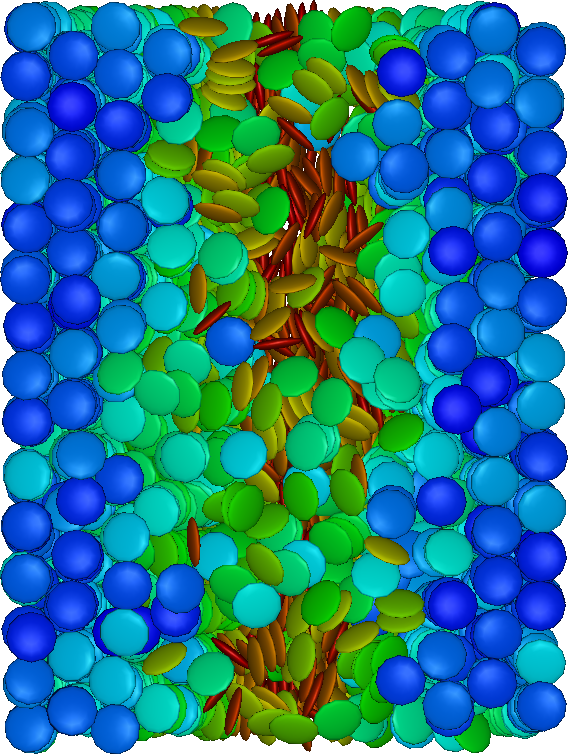
\includegraphics[width=.2\linewidth]{images/ceo_W8C8_D0.png}
 \qquad
 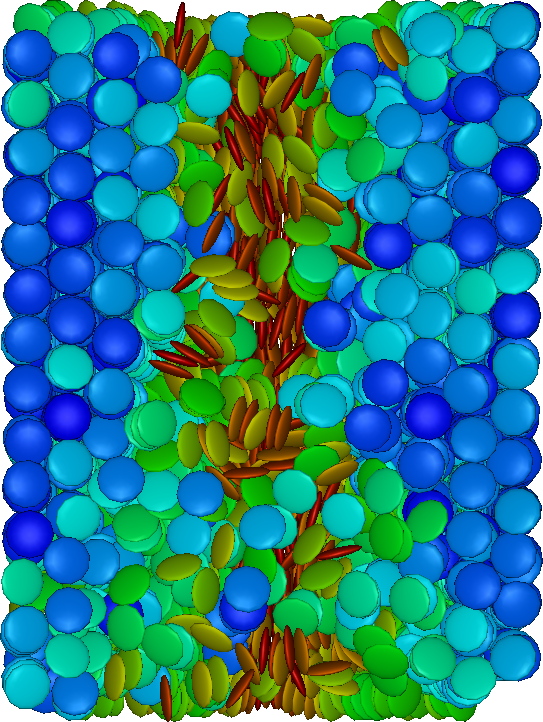
\includegraphics[width=.2\linewidth]{images/ceo_W8C8_D3.png}
 \qquad
 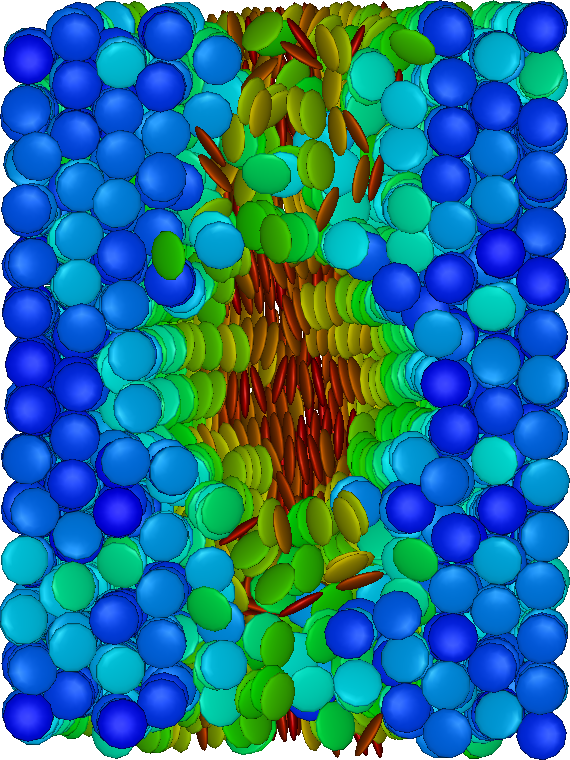
\includegraphics[width=.2\linewidth]{images/ceo_W8C8_D6.png}
 \qquad
 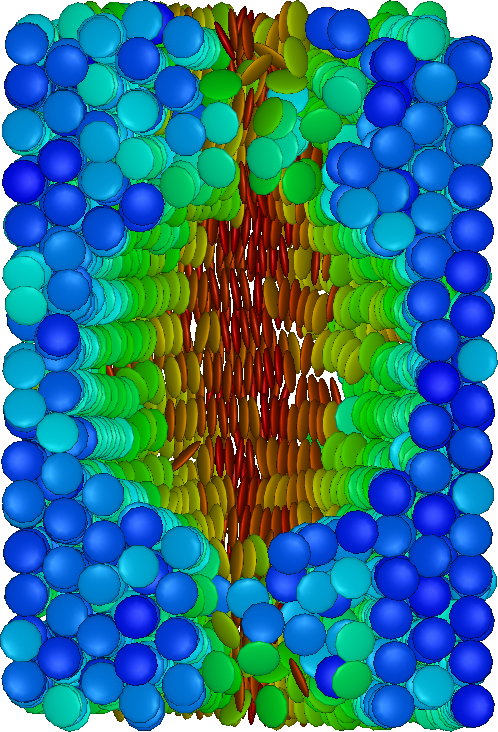
\includegraphics[width=.2\linewidth]{images/ceo_W8C8_D9.png}
 \caption{Cross sectional snapshots of the confined discotic liquid crystal system at $P^* = 50$, $T^* = 5.0$ with no colloid (far left), and with colloids of diameter $D^* \in \{3,6,9\} $. The pore diameter is $11.25\sigma_{ee}$.}
 \label{fig:confsnapshots}
\end{figure}
We studied the behaviour of the system through the various order parameters introduced in the previous sections. 
Figure \ref{fig:ceoC8nemloc} shows the dependence of the local nematic order parameter on the temperature. We can see a quantized assembly of rings as found by Sentker, Zantop \cite{sentker2018quantized} happening for every size of colloids. However, we can also see that as the colloidal size increases, the transitions happen at higher temperature and that the meta-stable plateaus appearing for smaller colloids become more sloped and the transitions become more soft. In the inset figure we can see that the assembly does not change significantly for colloids of diameter less than $D^* < 5$.


\begin{figure}[H]
    \centering
	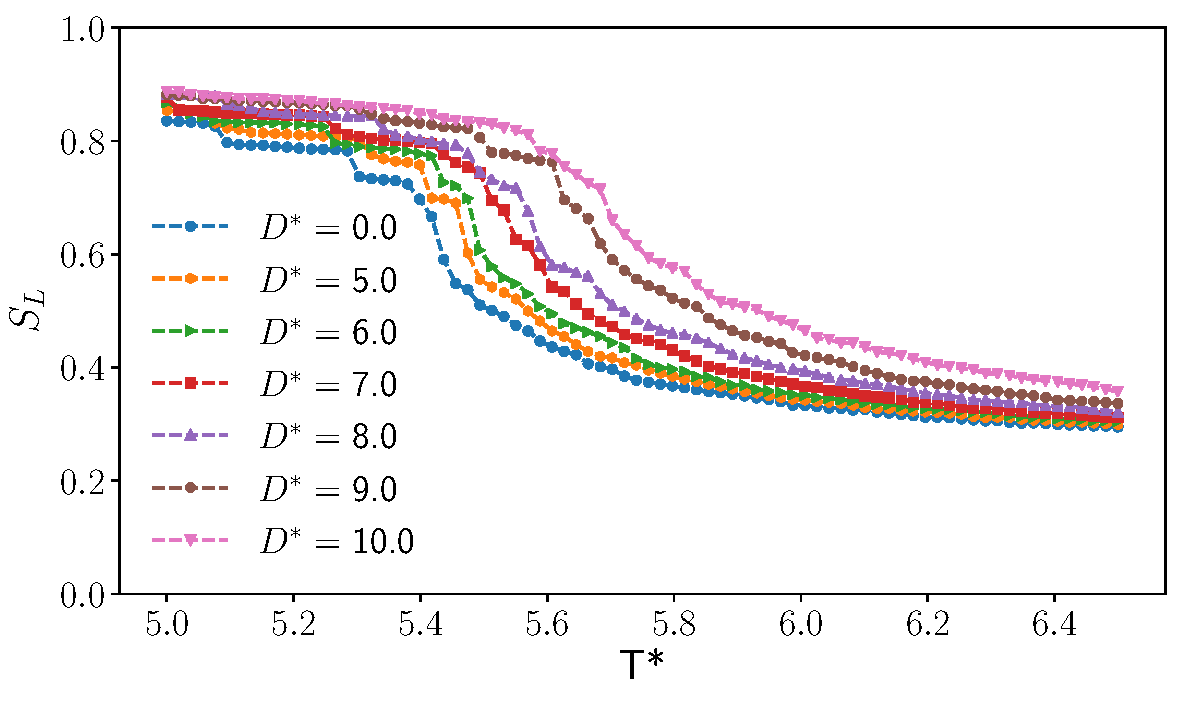
\includegraphics[width=0.8\linewidth]{plots/ceo_W8C8_nemloc.pdf}
	\caption{Dependence of the local nematic order parameter on the temperature for confined systems with colloids of different size}
    \label{fig:ceoC8nemloc}
\end{figure}
To further study the transitions, we looked at the hexagonal order parameter which describes the columnar alignment of the rings, and the circular order parameter which describes the more general alignment along the concentric rings. 
Looking at the hexagonal order parameter we see more quantized transitions while the circular orientation
displays a similar behaviour to the local nematic order parameter which suggests that in the presence of a colloid, the circular concentric alignment of the molecules happens more continuously while the actual formation of columnar rings remains discrete.  

\begin{figure}[H]
    \centering
	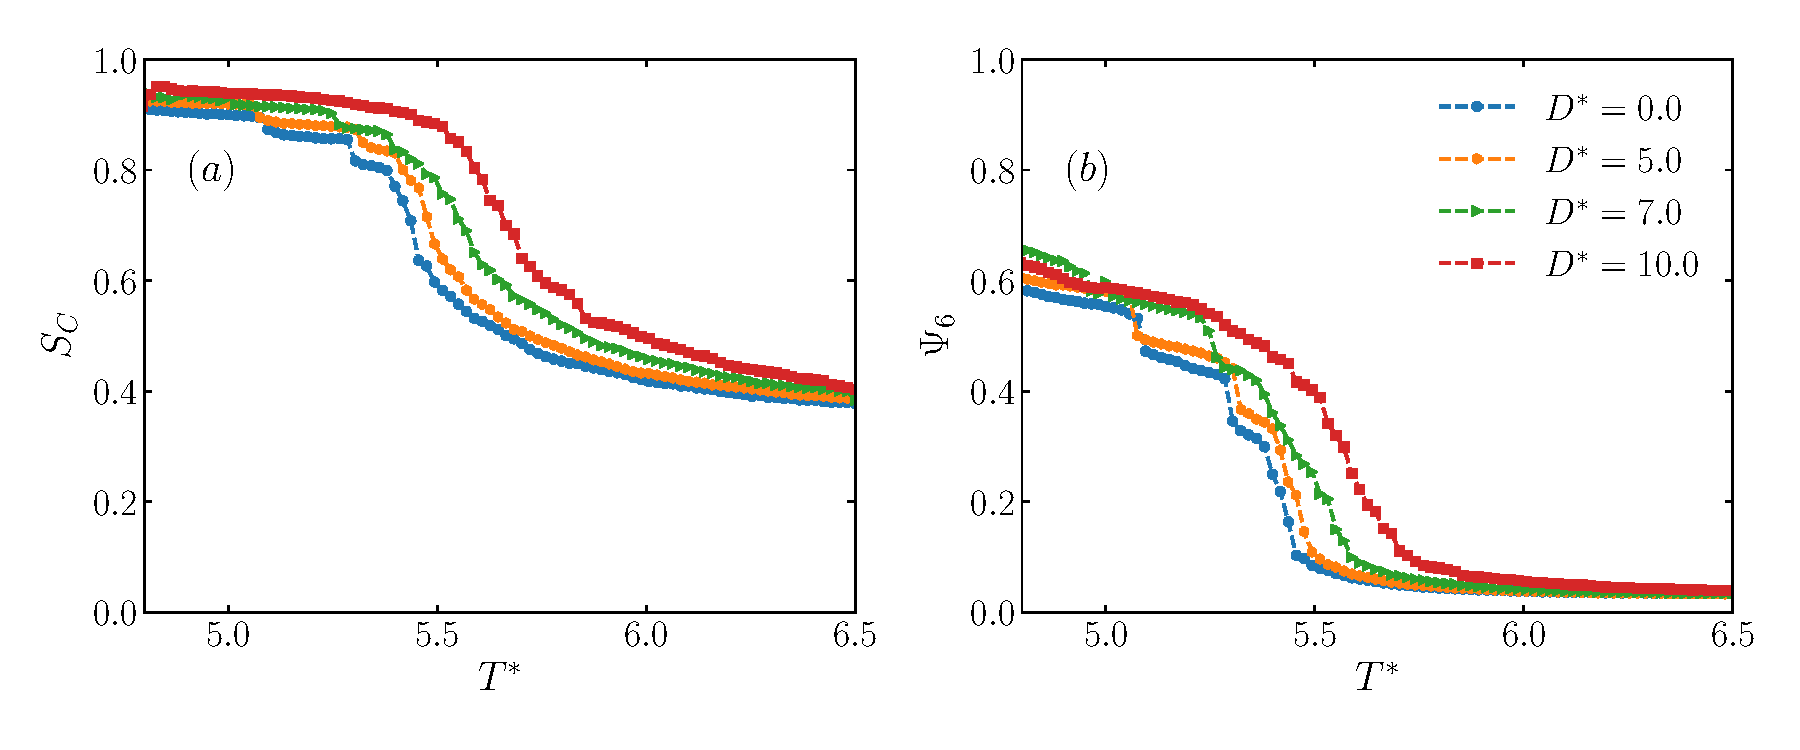
\includegraphics[width=\linewidth]{plots/ceo_W8C8_circhex.pdf}
	\caption{Dependence of the circular order parameter and the hexagonal order parameter  on the temperature for confined systems with colloids of different size}
    \label{fig:ceoC8hex}
\end{figure}

Figure \ref{fig:ceoC8raddens} shows the (2-D) radial density distribution
at different temperatures for 
Here we can see the concentric rings forming for a system with a colloid of diameter $D^*=8$ as the system cools down. We can see the particles assembling into columnar rings which are packed hexagonally, as evidenced by the high bond order in the outer rings. However as they approach the cylindrical axis, the order decreases, due to the coinciding line defect.

\begin{figure}[H]
    \centering
	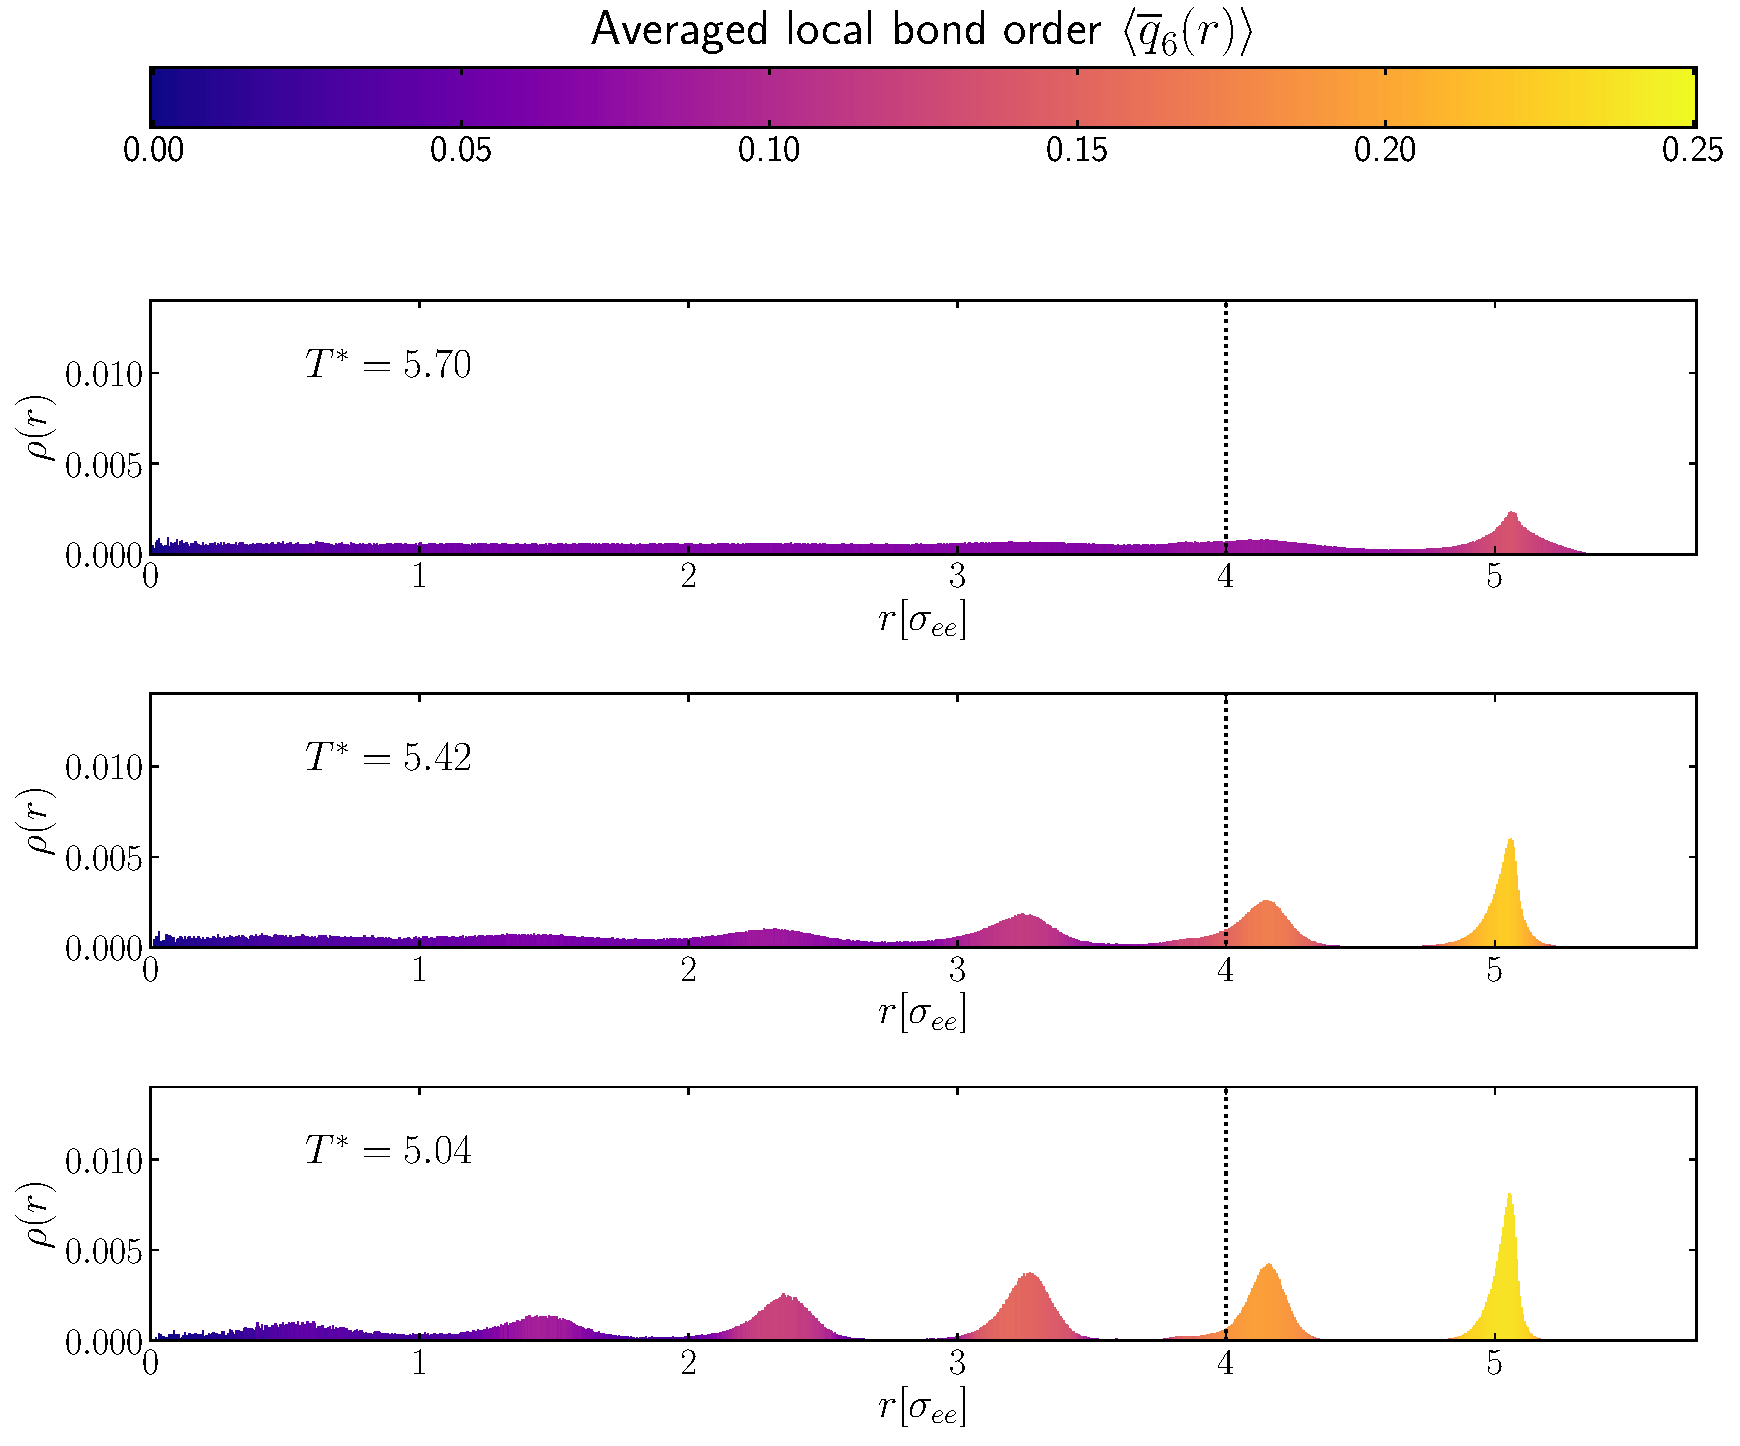
\includegraphics[width=0.8\linewidth]{plots/ceo_W8C8_raddensD8.pdf}
	\caption{Radial dependence of the local density and averaged bond order at different temperatures for a system with a colloid of diameter $D^* = 8$. The vertical dashed line represents the radius of the colloid.}
    \label{fig:ceoC8raddens}
\end{figure}




\subsection{Face-On Anchoring at $\epsilon_{\text{cf}}^*= 56$}


\begin{figure}[H]
 \centering
 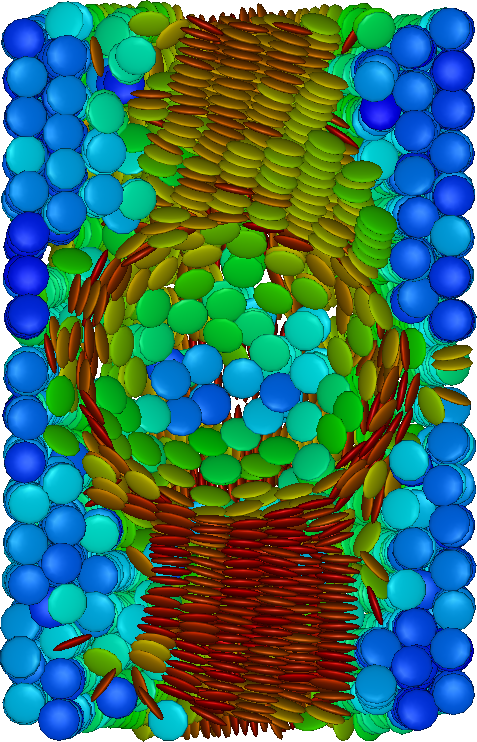
\includegraphics[width=.2\linewidth]{images/cfo_W8C56_D7.png}
\caption{Cross sectional snapshots of the confined discotic liquid crystal system at $P^* = 50$, $T^* = 3.7$ with colloids of diameter $D^*=7 $.}
 \label{fig:cfosnapshots}
\end{figure}

We can see from Figure \ref{fig:cfosnapshots} that the imposed structure from the pore is not compatible with the imposed structure from the colloid with the face-on anchoring. We can see discotic particles forming a single layer around the colloid, which leads to axially aligned logpile configurations along the cylindrical axis.


Looking at the local nematic order parameter in function of the temperature in Fig. \ref{fig:cfonemloc}, we see, that the nature of the transition does not change, which however is shifted towards colder temperatures, as the colloid grows in diameter.


\begin{figure}[H]
    \centering
	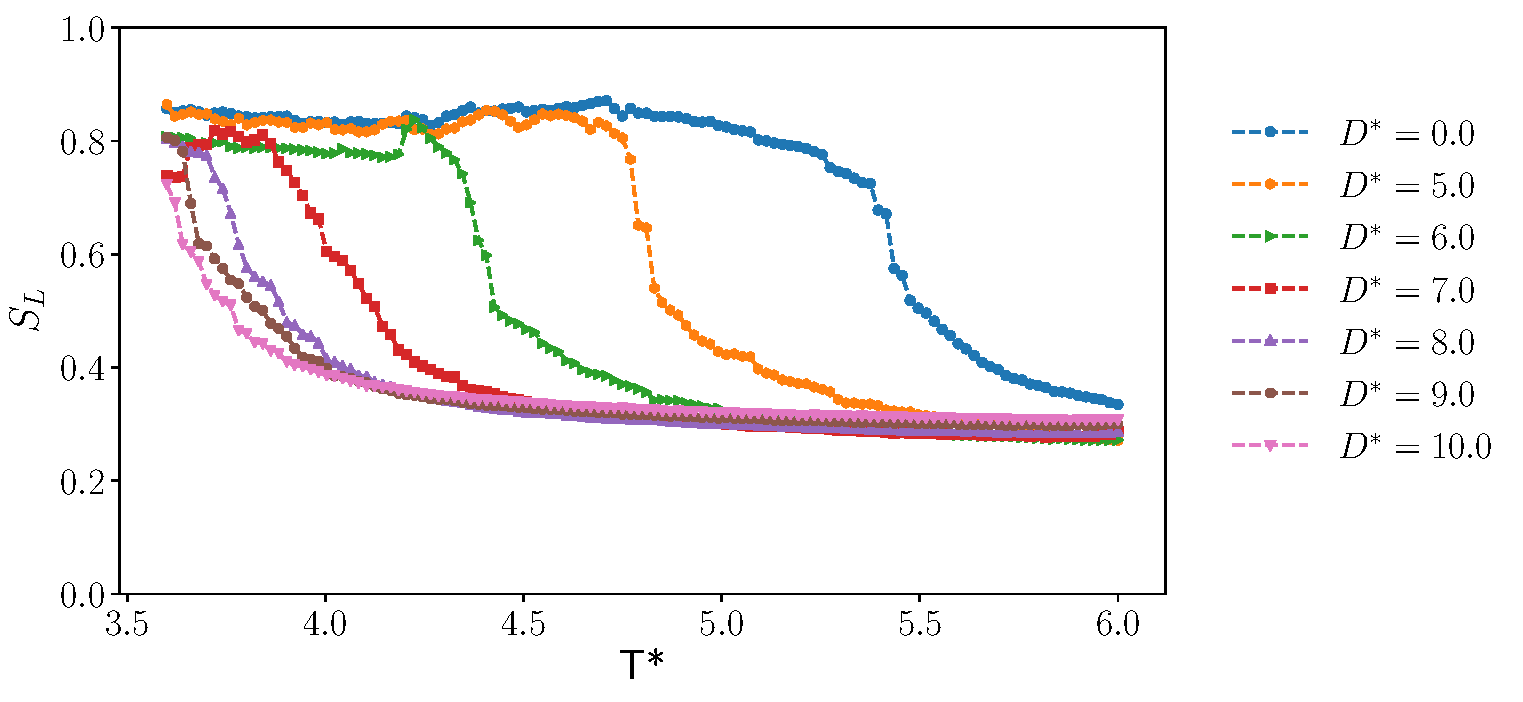
\includegraphics[width=\linewidth]{plots/cfo_W8C56_nemloc.pdf}
	\caption{Dependence of the local nematic order parameter on the temperature for systems in bulk with colloids of different size}
    \label{fig:cfonemloc}
\end{figure}
\begin{figure}[H]
    \centering 
	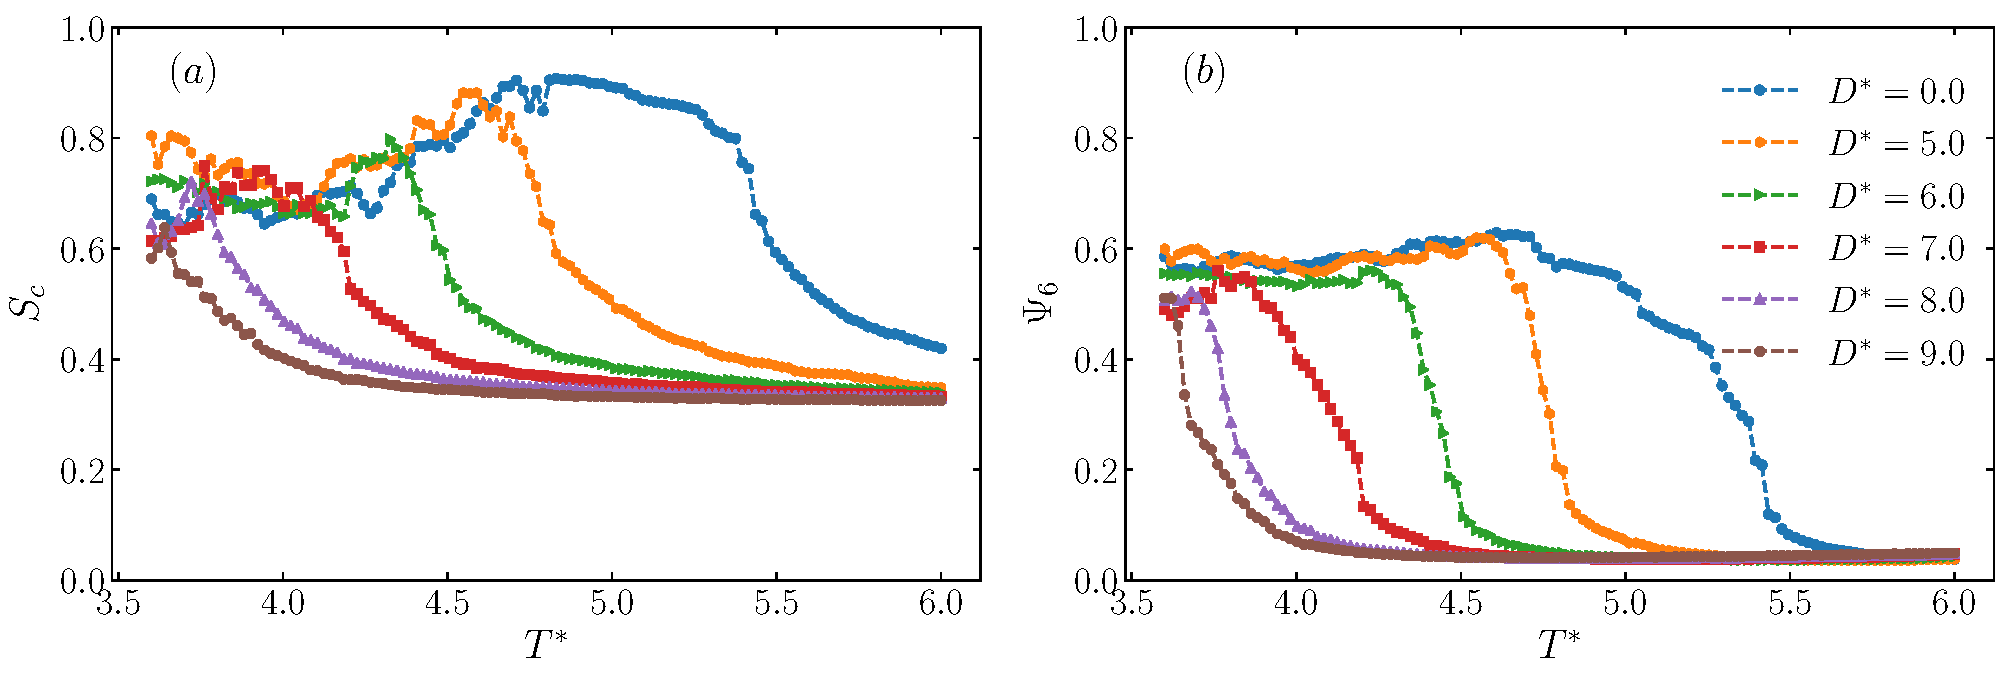
\includegraphics[width=\linewidth]{plots/cfo_W8C56_hexcirc.pdf}
    \caption{Dependence of the hexagonal (a) and  circular nematic parameter (b)  on the temperature for systems in bulk with colloids of different size.}
    \label{fig:cfohexcirc}
\end{figure}


Cooling the system even further down the inner rings break up and the aforementioned coaxially aligned logpile configurations form, which can be seen by the drop in circular nematic order at lower temperatures in Figure \ref{fig:cfohexcirc}, whereas the local nematic order and hexagonal order stay fixed. If we look at the radial density of a system with a colloid of size $D^*=6$ in Fig. \ref{fig:cforaddens} we can see the formation of the concentric outer rings but we can also see the formation of the inner configuration, since the most inner density peaks are broader and there is higher structural order in the inner layer of the pore, indicating the absence of a line defect in this configuration.

\begin{figure}[H]
 \centering
 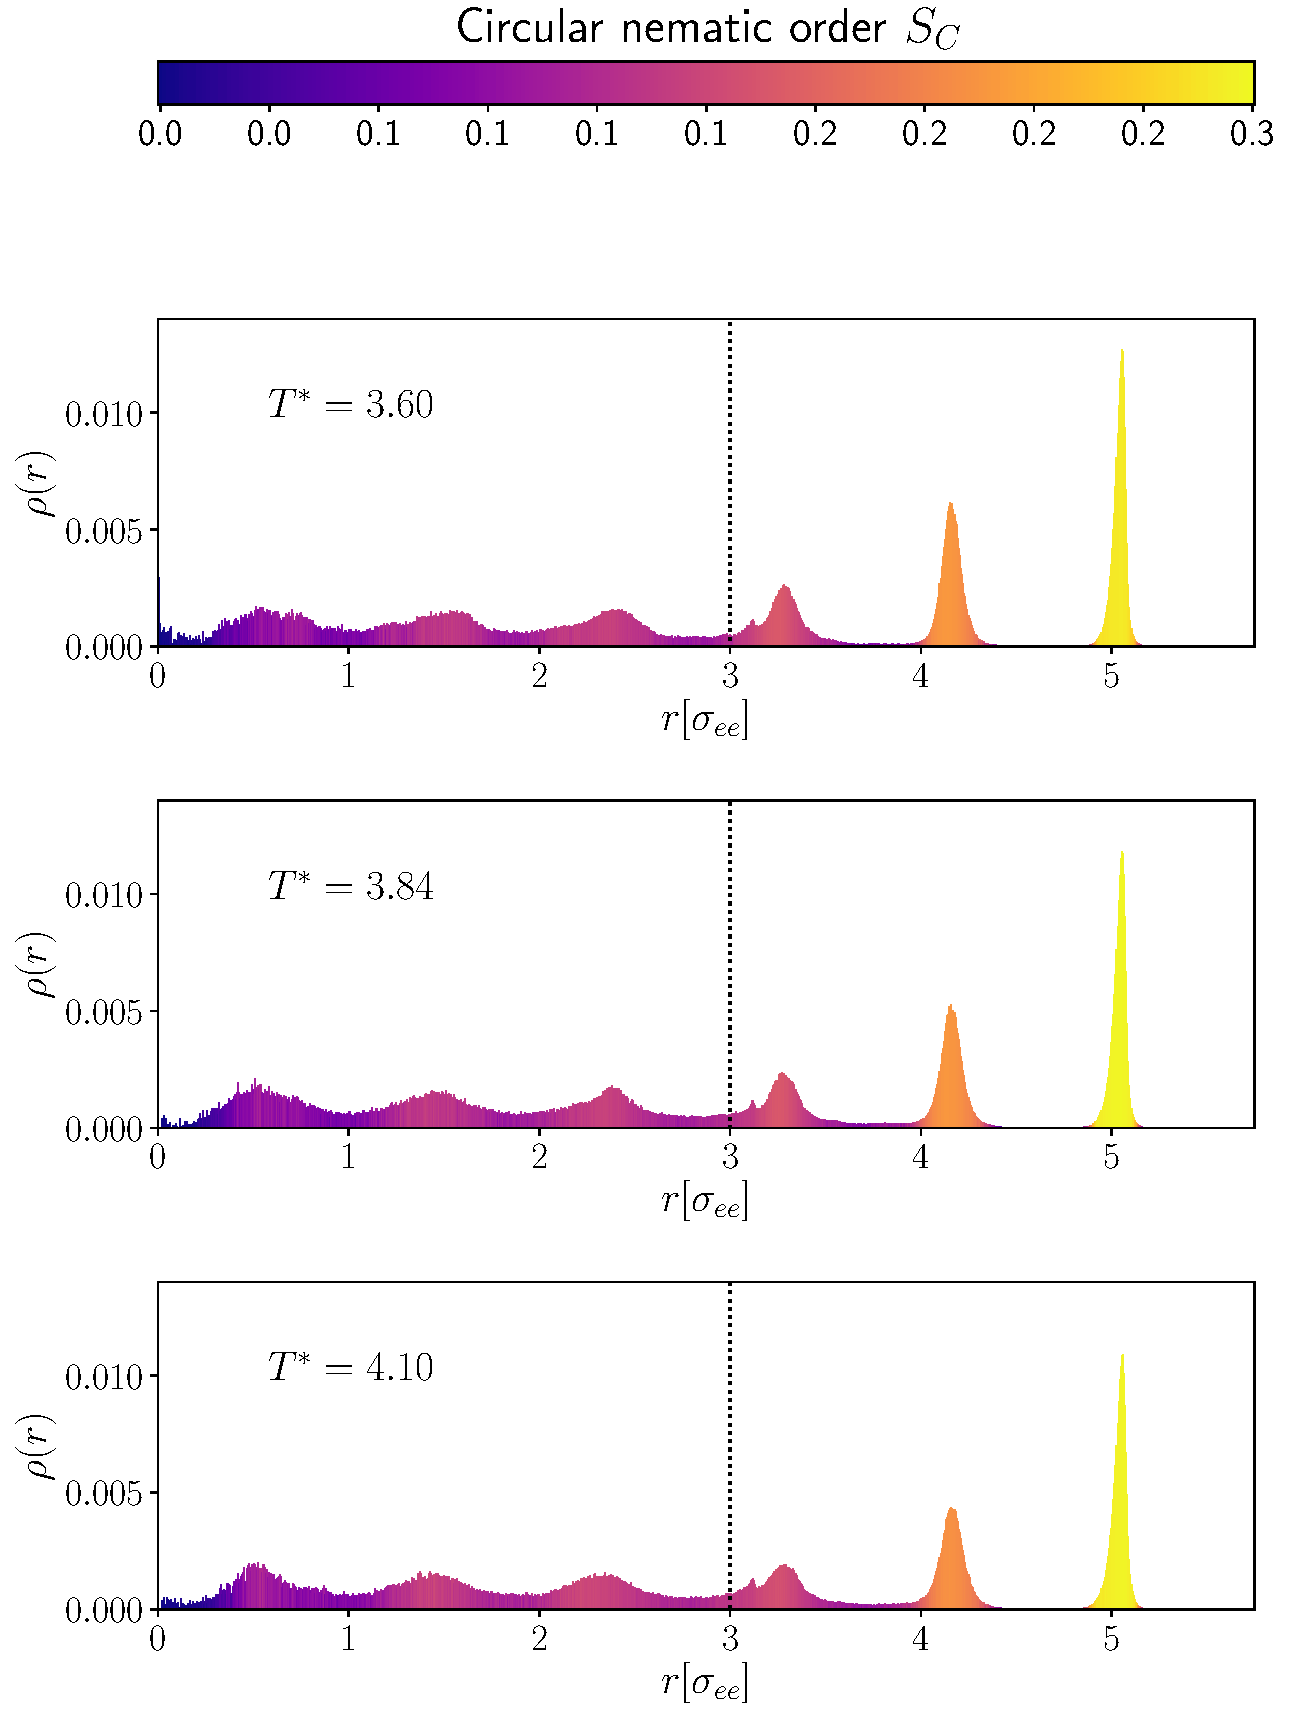
\includegraphics[width=0.8\linewidth]{plots/cfo_W8C56_raddensD6.pdf}
\caption{Radial dependence of the local density and circular nematic order at different temperatures for a system with a colloid of diameter $D^* = 6$ (right). The vertical dashed line represents the radius of the colloid.}
 \label{fig:cforaddens}
\end{figure}




\section{Bulk}
\label{sec:Bulk}
To study the system in bulk we imposed periodic boundary conditions and set a colloidal particle of diameter $D^* \, [\sigma_{ee}]$ in the centre of the system. To try to avoid any small system effects due to the periodic boundary conditions, we had to simulate 10000 particles to offset the size of the colloid, the diameter of which ranges from $5$ to $10$. As in the confined case, most effects start appearing only for colloids of diameter $D^* \geq 6$. As the number of particles increases, the number of performed equilibration steps must also increase, so as to ensure that the sampling steps are representative for the probability distribution. This however increases the simulation time. To compensate for this we decreased the temperature resolution, only increasing it in the vicinity of the transition.

\iffalse
This takes quite some time (between one and two weeks for one batch of simulations) since the range of temperatures has to be fairly precise so as to avoid any weird effects happening, and the number of performed equilibration steps needs to be increased with the number of particles. therefore the results here are not as complete as I would prefer. In particular the plots of the (global) nematic order parameter in function of the temperature are very noisy, due to the appearance of locally aligned groups of molecules. This could be solved with an even longer run-time, and maybe a few optimizations in the code, which of course would take even longer to run.
\footnote{One possible way to artificially reduce the necessary particle number is to choose a different shape for the simulation box, e.g. a truncated octahedron, that has better sphericity. However, I suspect the box would have to be a regular polyhedron, which may be a disadvantage due to the irregular shape of the particles.}
\fi
\subsection{Edge-On Anchoring at $\epsilon_{\text{cf}}^*= 32$}

\begin{figure}[H]
 \centering
 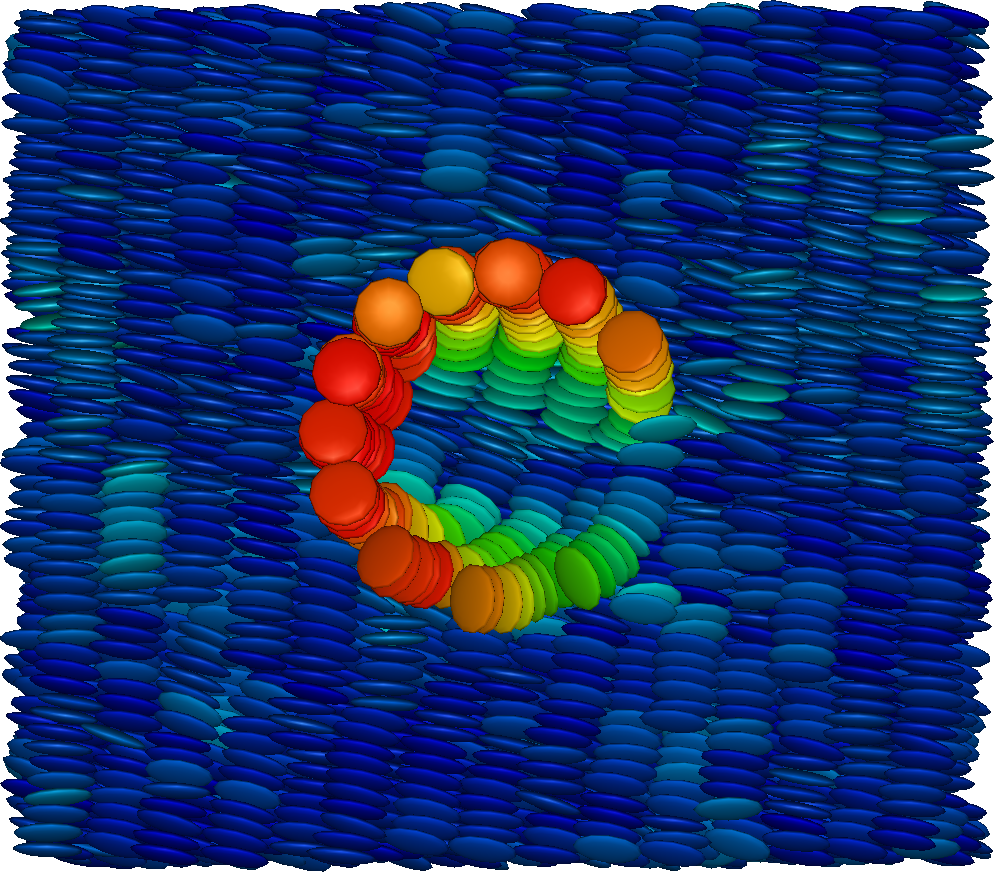
\includegraphics[width=.4\linewidth]{images/beo_C32_D5.png}
 \qquad
 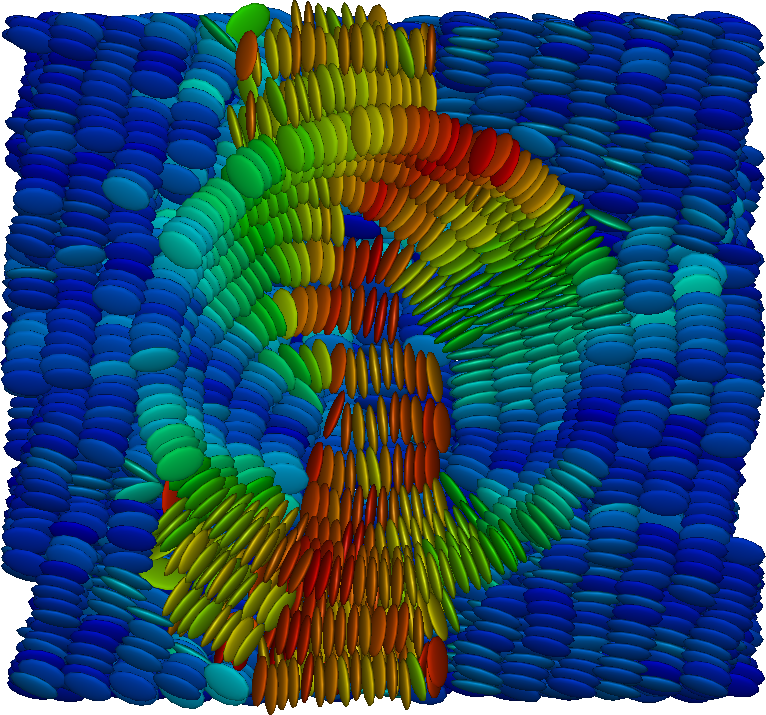
\includegraphics[width=.4\linewidth]{images/beo_C32_D9.png}
\caption{Cross sectional snapshots of the bulk discotic liquid crystal system at $P^* = 50$, $T^* = 4.6$ with colloids of diameter $D^* \in \{5,9\} $.}
 \label{fig:beosnapshots}
\end{figure}


Imposing edge-on anchoring on the colloid we can see in Fig. \ref{fig:beoc32lochex} that the phase transition becomes continuous with the introduction of the colloid. Whereas the bulk system without a colloid displays a first order transition the introduction of a colloid smoothens the transition, giving it a more gradual progression. We can also see that the magnitude of the order parameters in the columnar phase decrease with respect to the colloid size, which is probably due to the layer of discotic particles around the colloid at most temperatures and colloid sizes.
\begin{figure}[H]
    \centering
	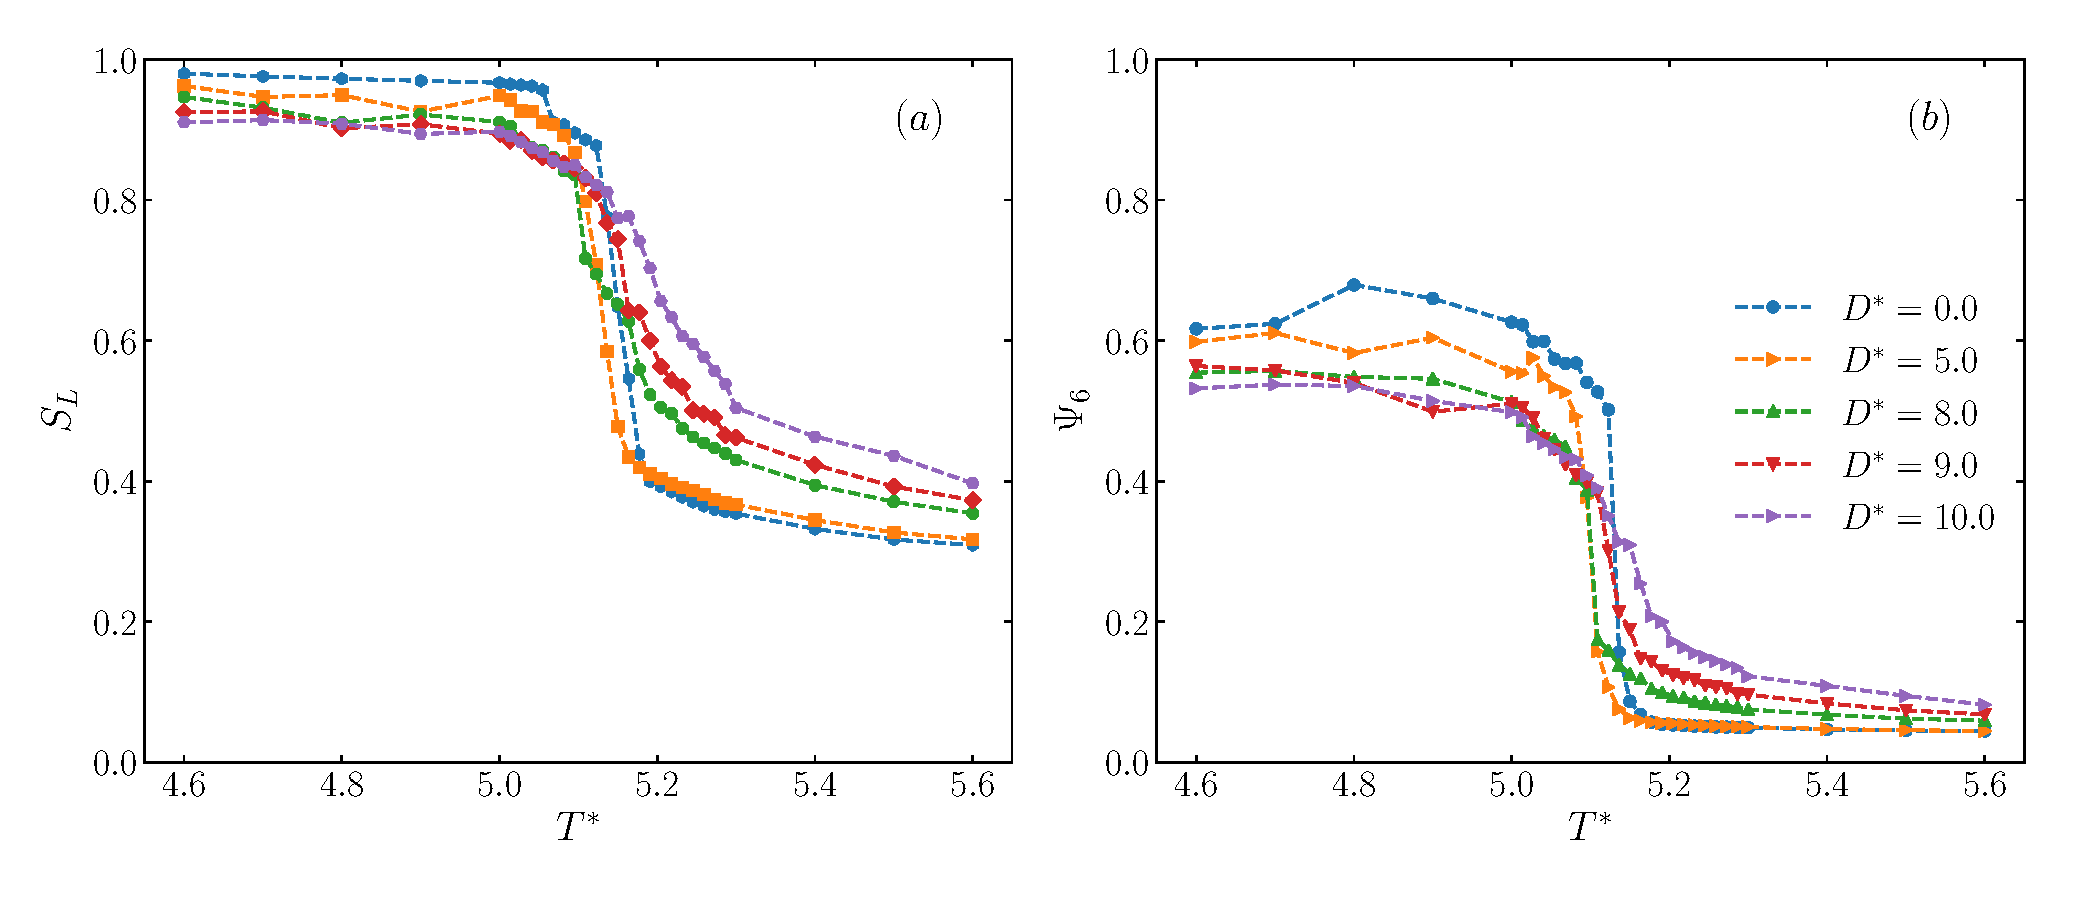
\includegraphics[width=\linewidth]{plots/beo_C32_lochex.pdf}
	\caption{Dependence of the local nematic order parameter and the hexagonal on the temperature for systems in bulk with colloids of different size.}
    \label{fig:beoc32lochex}
\end{figure}
We can study the structural properties in more detail with the help of the radial distribution function. Fig. \ref{fig:beoc32rdf} shows the parallel and the perpendicular for two exemplary cases.  
\begin{figure}[H]
    \centering
	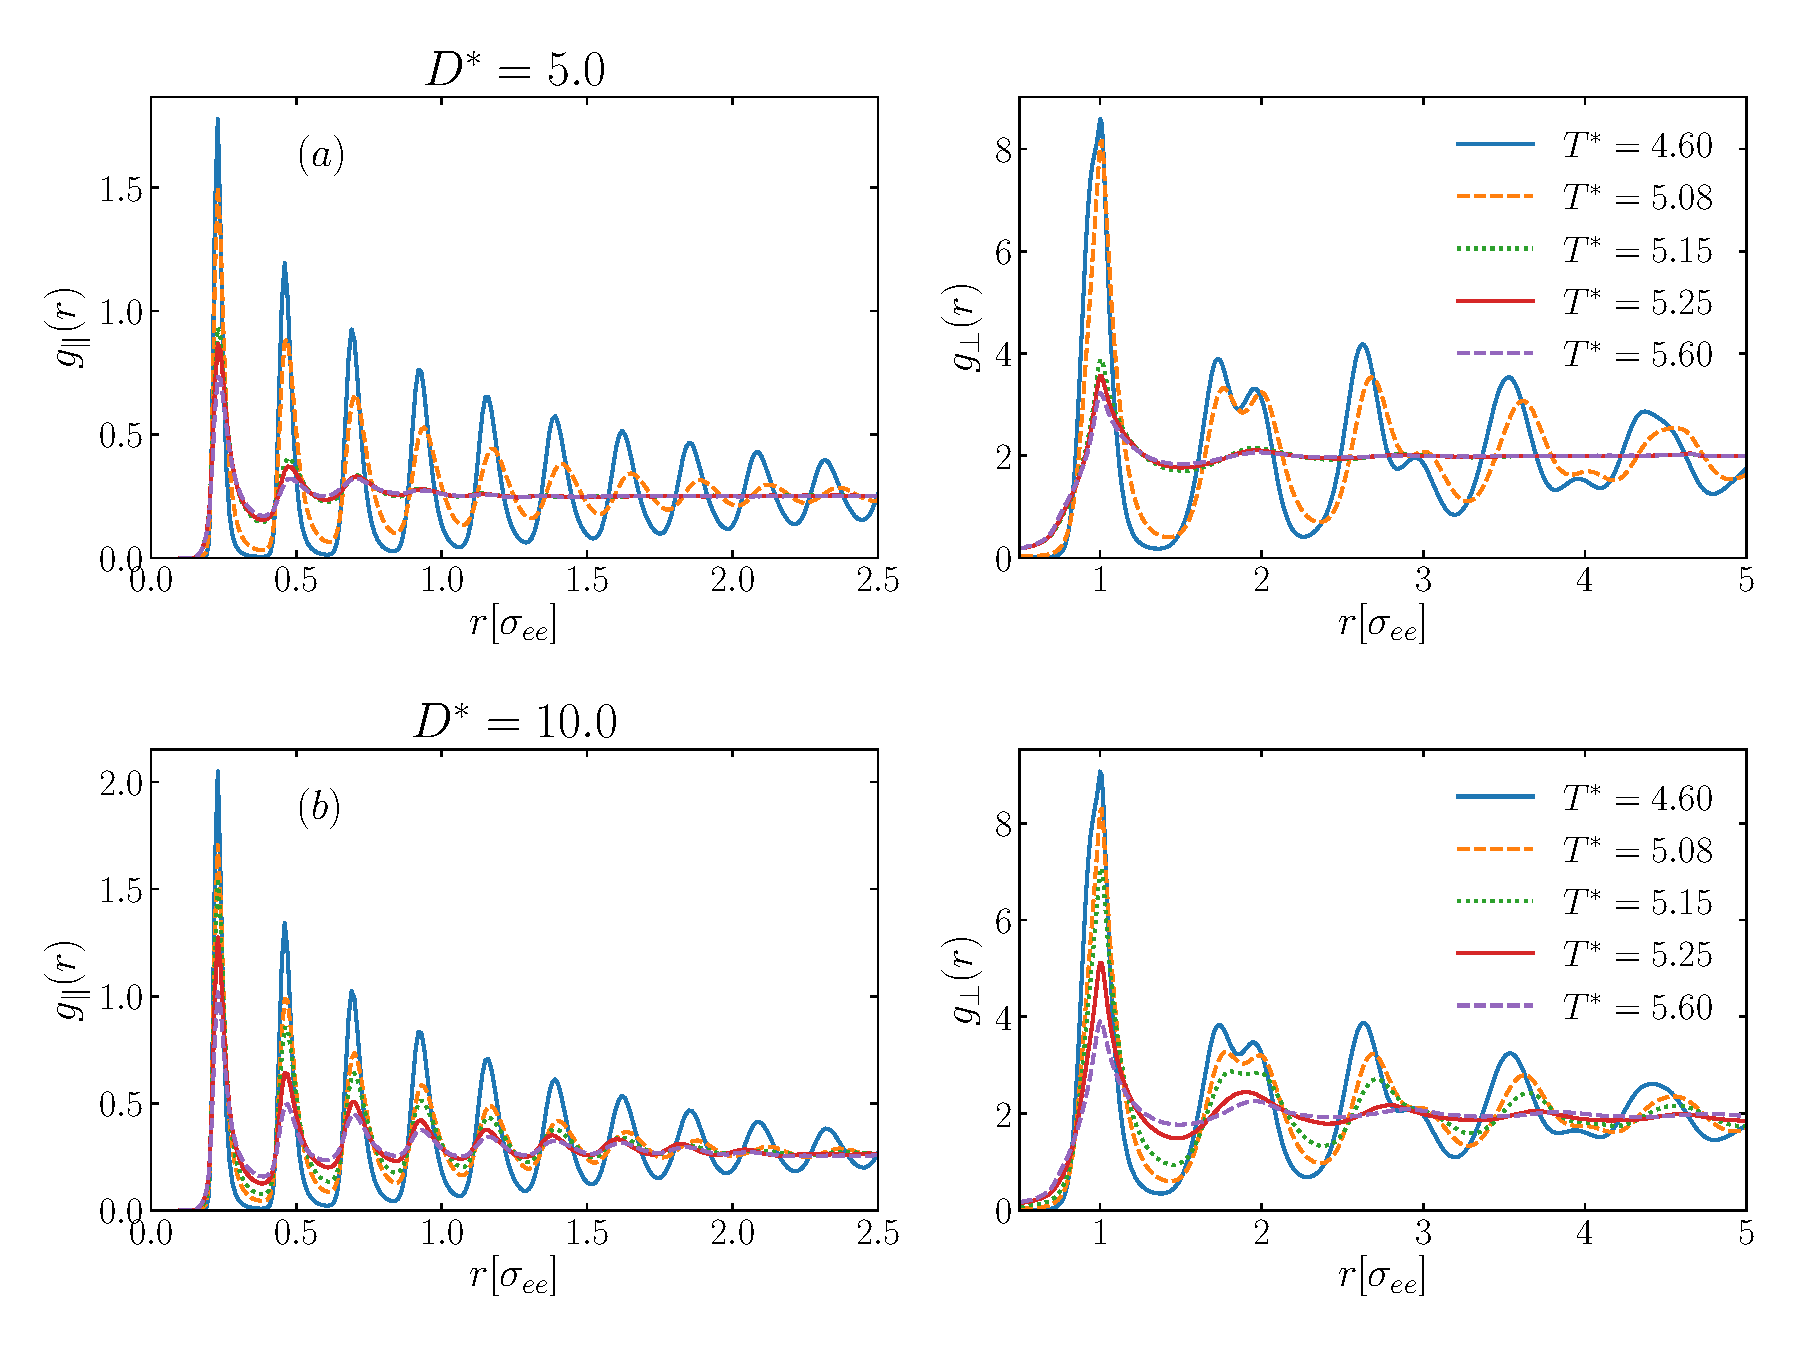
\includegraphics[width=\linewidth]{plots/beo_C32_rdf.pdf}
	\caption{Radial distribution function at different temperatures of a system with colloids of sizes $D^* =  5$ (a) and $D^* = 10$ (b).}
    \label{fig:beoc32rdf}
\end{figure}
We can see the phase transition from the isotropic to the columnar in the structural change of the perpendicular RDF. While the transition is sudden for the system with the colloid of diameter $D^*=5$ (a), we can confirm that for a bigger colloid, the transition happens continuously.
The presence of the colloid lends itself to examine the structure more closely, using the average bond order parameter to determine the local structure as a function of the distance towards the center. For the colloid of diameter $D^*=5$ there are no real local heterogeneities, except for the slight accumulation of particles on the colloidal surface.
Looking at the local bond order of the system with a colloid of diameter $D^*=10$ we can see that as the system cools down, layers around the colloid start forming. As it is impossible for the discotic particles to cover the surface of the colloid without any defects with an edge-on alignment, these layers cannot achieve the same sharpness as in the confined case.


\iffalse
If we look at the local radial density in Figure 6 we can see at least one distinct layer of particles near the colloid forming. For the larger colloids we can see the formation of distinct layers that form in the early stages of the columnar phase that start breaking up at lower temperatures due to the tendency of alignment towards the nematic director.
\fi

\begin{figure}[H]
    \centering
	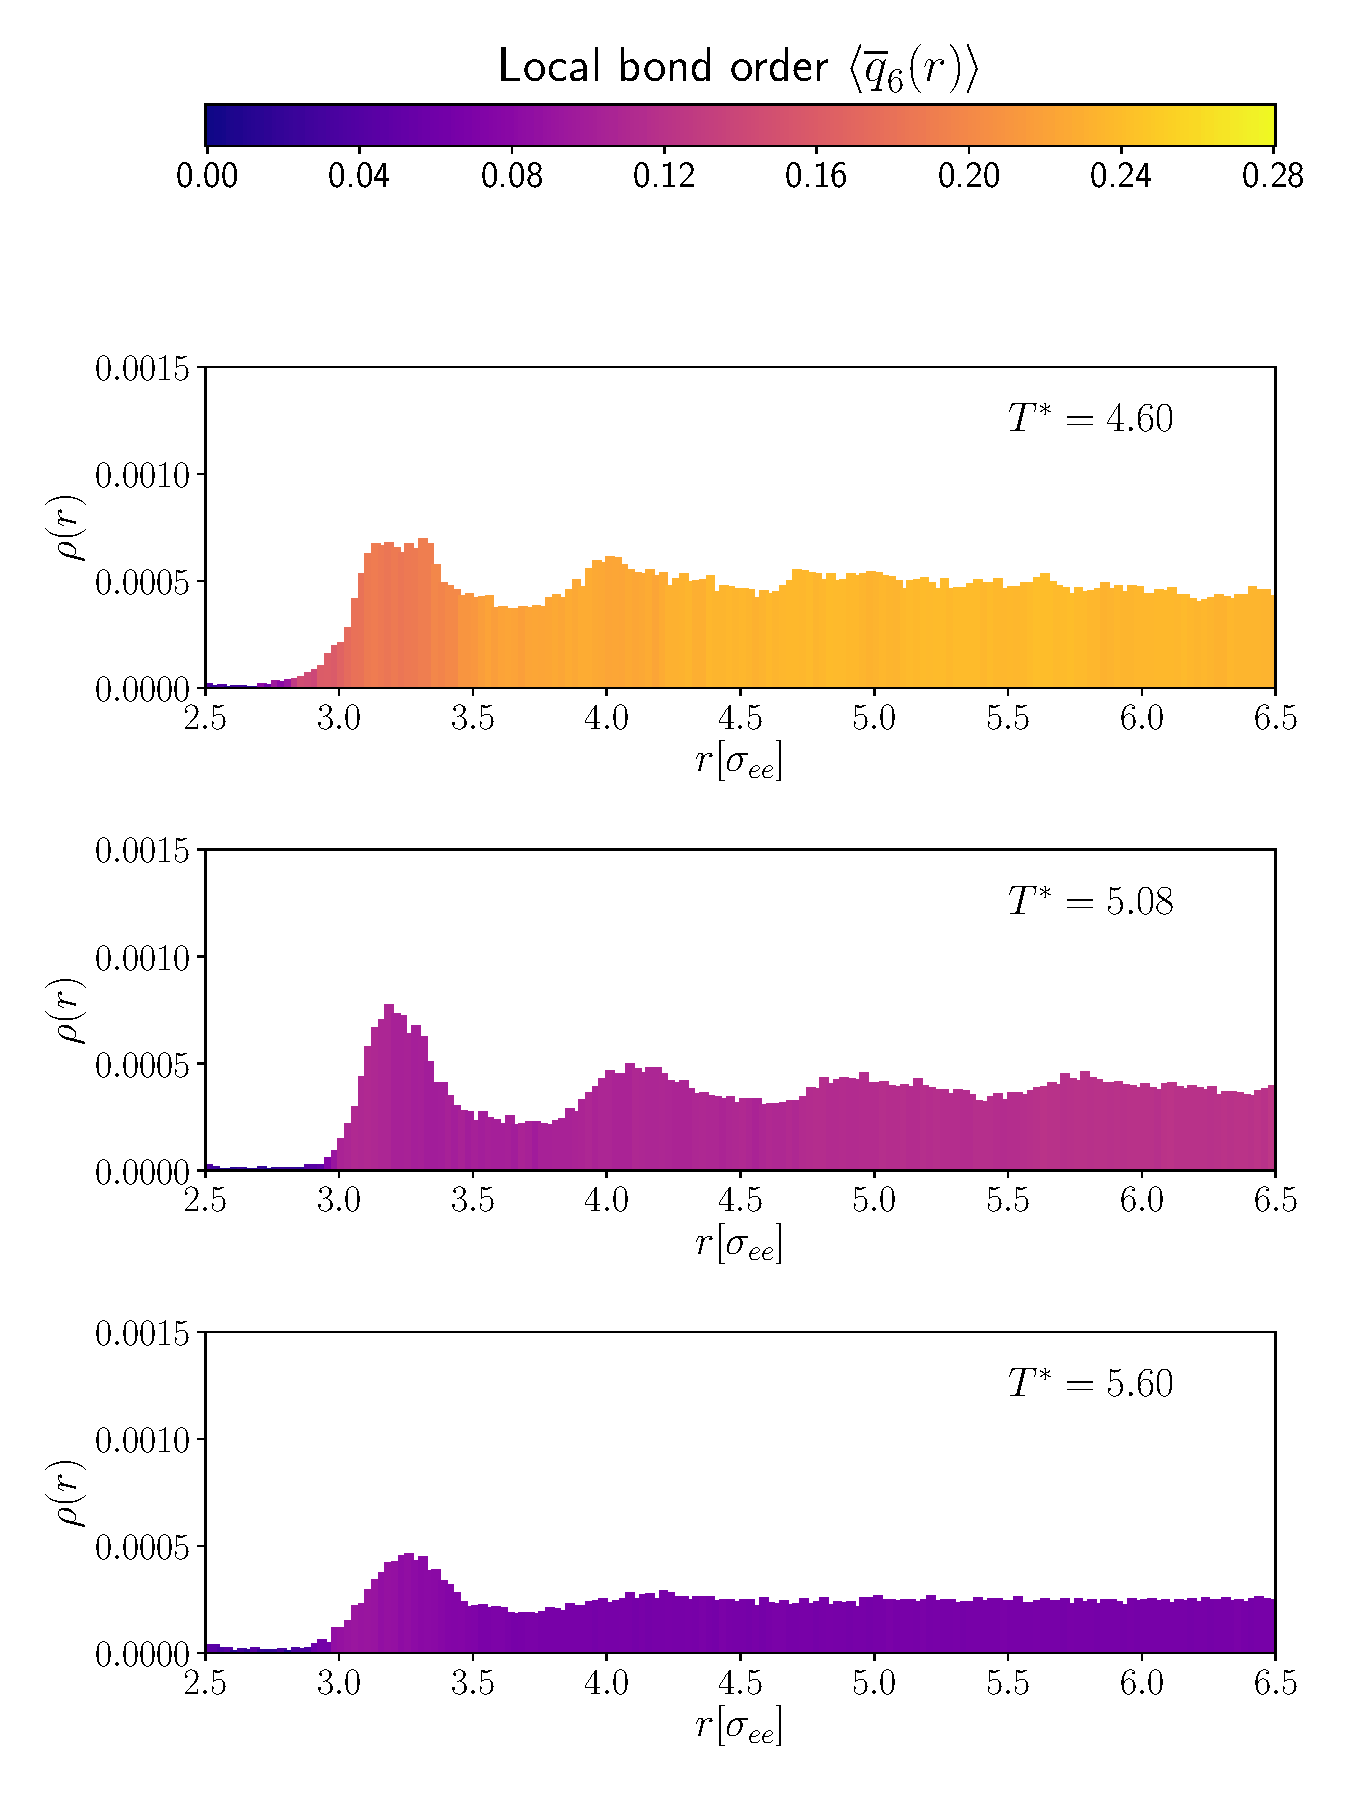
\includegraphics[width=0.49\linewidth]{plots/beo_C32_raddensD5.pdf}
	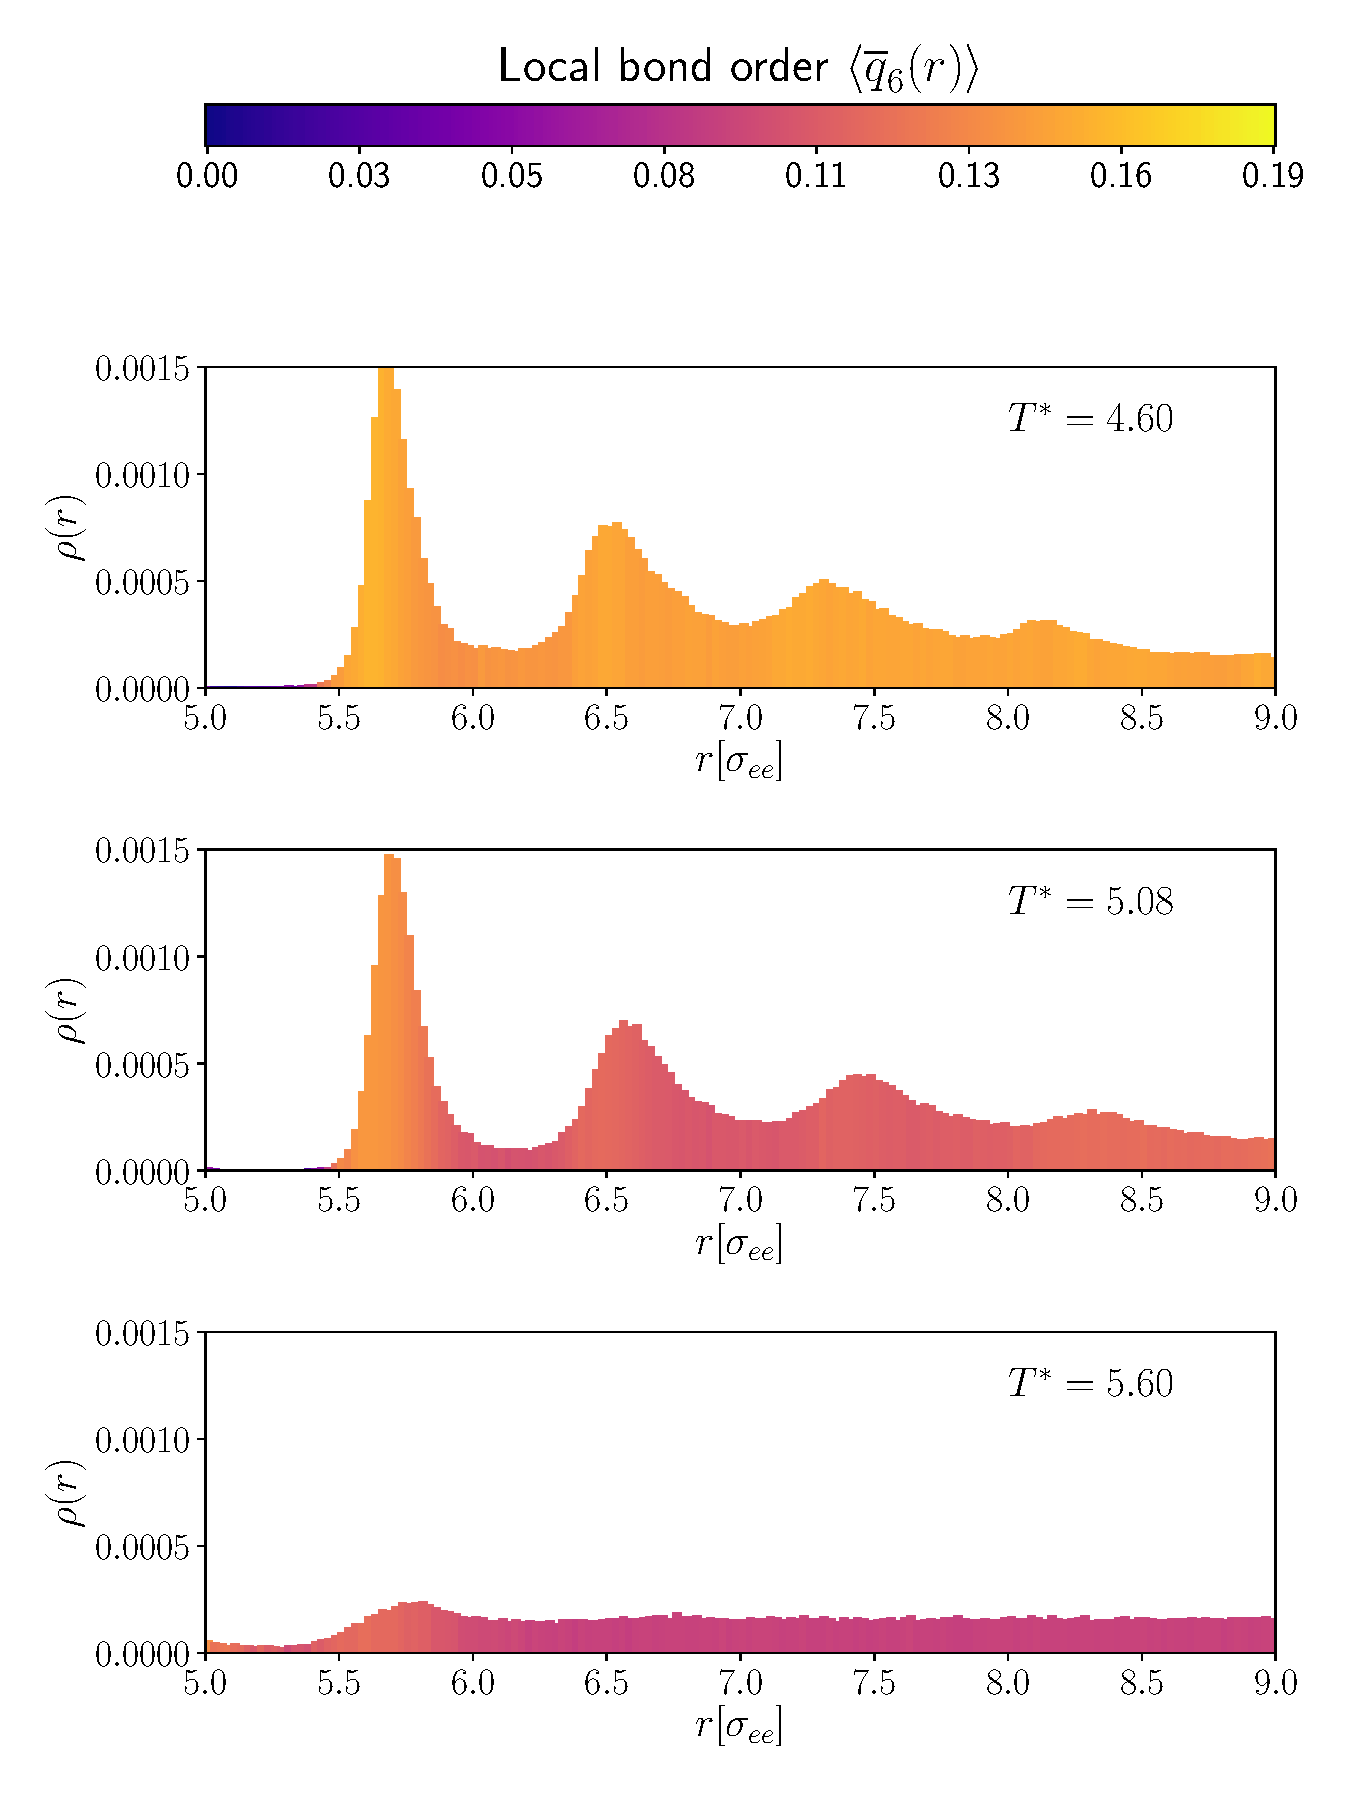
\includegraphics[width=0.49\linewidth]{plots/beo_C32_raddensD10.pdf}
	\caption{Radial dependence of the local density and bond orientational order parameter $ \overline{q}_6$ at different temperatures of a system with colloids of sizes $D^* =  5$ (a) and $D^* = 10$ (b)}
    \label{fig:beoc32nemloc}
\end{figure}

\subsection{Face-On Anchoring at  $\epsilon_{\text{cf}}^*= 56$}

 We finally studied face-on anchoring in bulk conditions.
\begin{figure}[H]
 \centering
 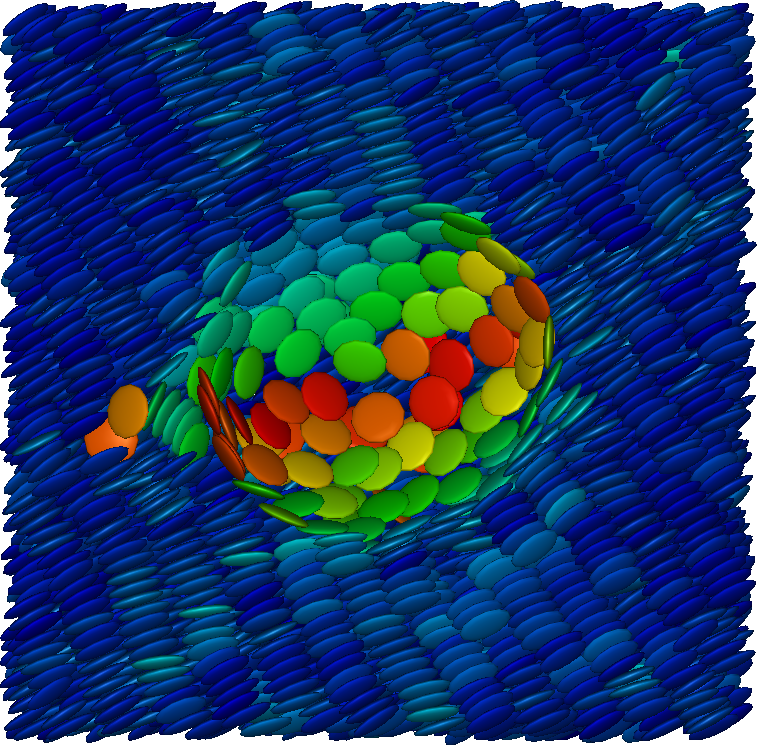
\includegraphics[width=.4\linewidth]{images/bfo_C80_D6.png}
 \qquad
 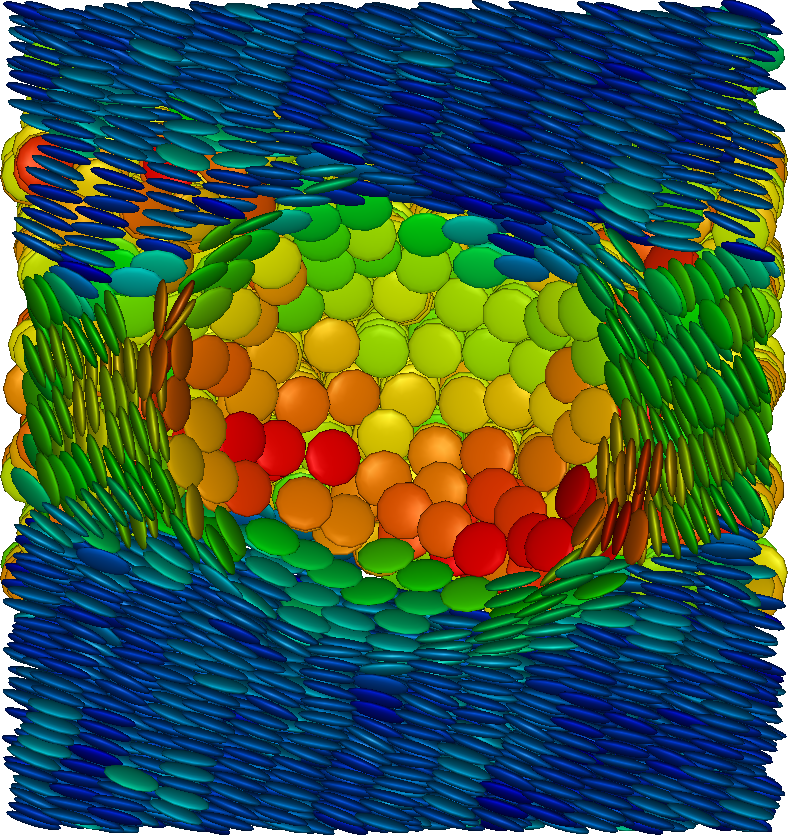
\includegraphics[width=.4\linewidth]{images/bfo_C80_D8.png}
\caption{Cross sectional snapshots of the bulk discotic liquid crystal system at $P^* = 50$, $T^* = 4.5$ with colloids of diameter $D^* = 6$ and $D^*=8$. }
 \label{fig:bfosnapshots}
\end{figure}
In Fig. \ref{fig:bfosnapshots} we can see some snapshots of example systems. We can see that the particles form a layer around the colloid, which, depending on the size of the colloid can lead to the formation of patches of locally aligned particles. It seems that again, the size of the colloid plays a very big role in the effect on the phase transition.
Looking at the local nematic order parameter in Fig. \ref{fig:bfoc32lochex} we can indeed confirm, that the colloid plays a minimal role if the diameter $D^*$ is smaller than $5$. For bigger colloids, the phase transition seems to be split into two discontinuous jumps in the approximately same temperature regime as without a colloid.

\begin{figure}[H]
    \centering
	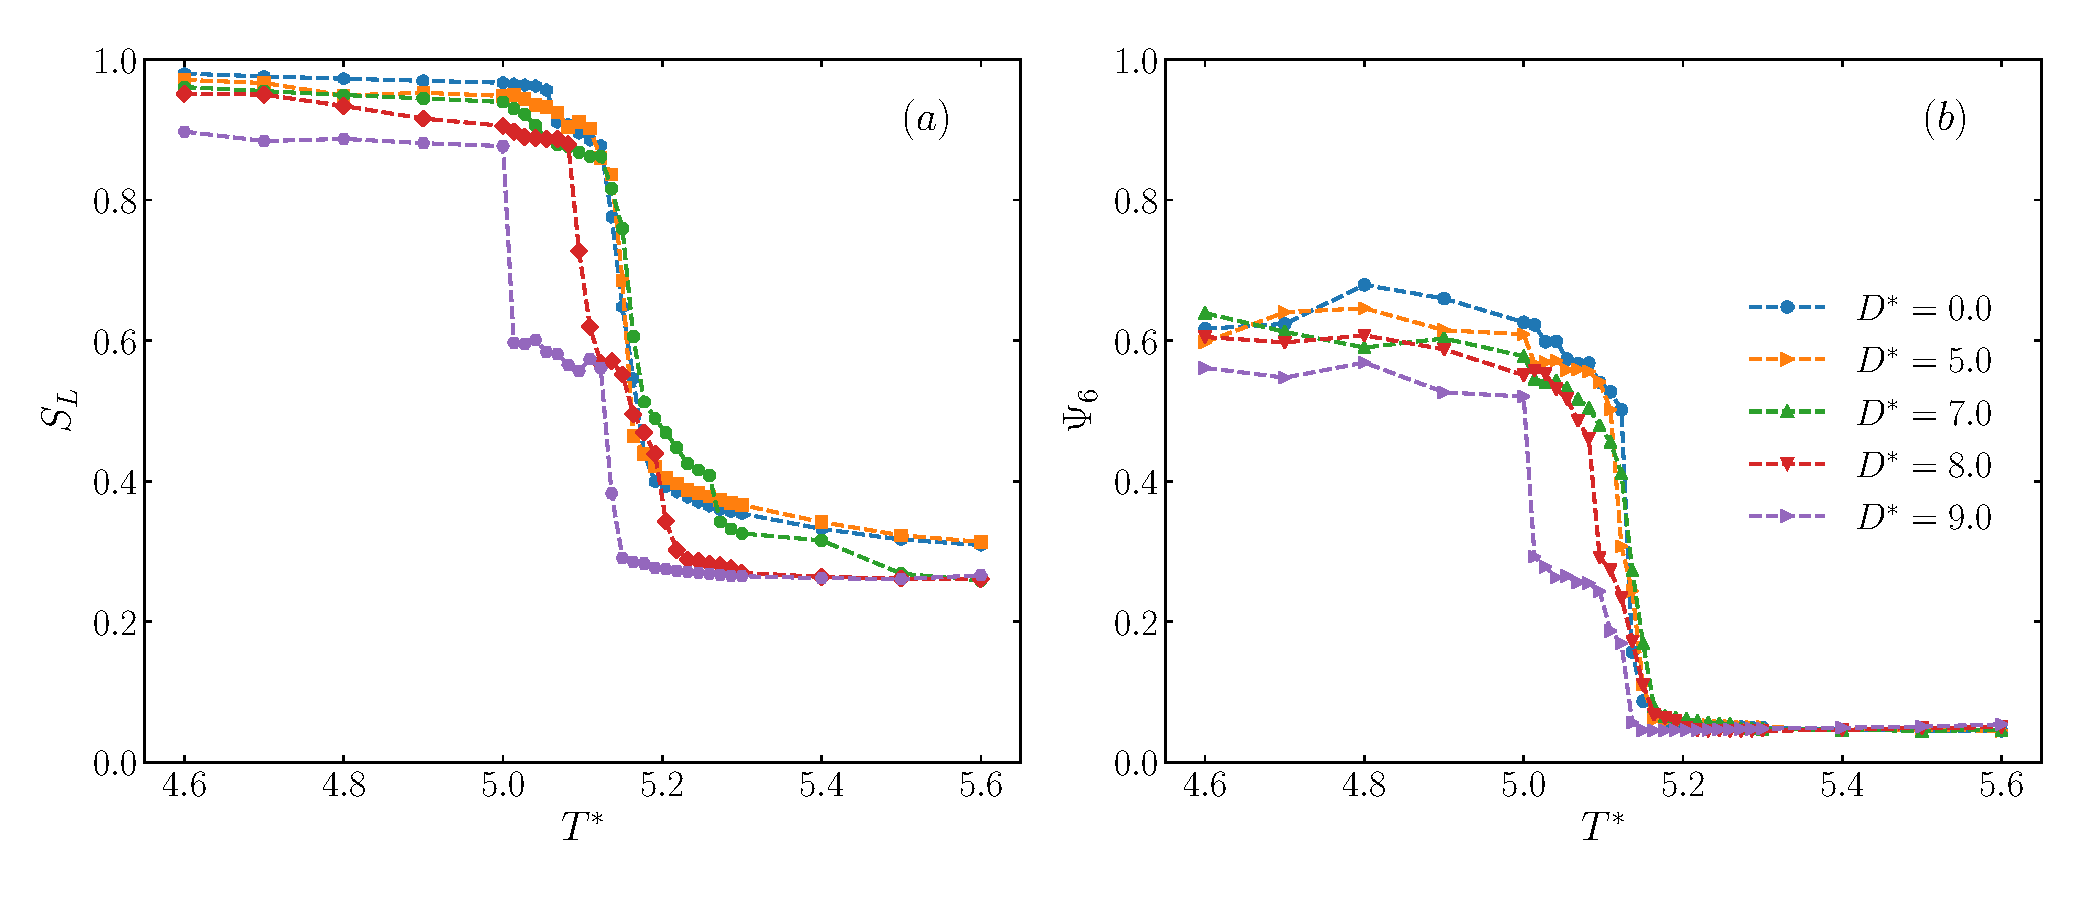
\includegraphics[width=\linewidth]{plots/bfo_C56_lochex.pdf}
	\caption{Dependence of the local nematic order parameter and the hexagonal on the temperature for systems in bulk with colloids of different size}
    \label{fig:bfoc32lochex}
\end{figure}

Looking at the local bond order and radial density in Fig. \ref{fig:beoc32raddens}, we can identify the reason for this appearance of a two-phase jump. 

\begin{figure}[H]
    \centering
	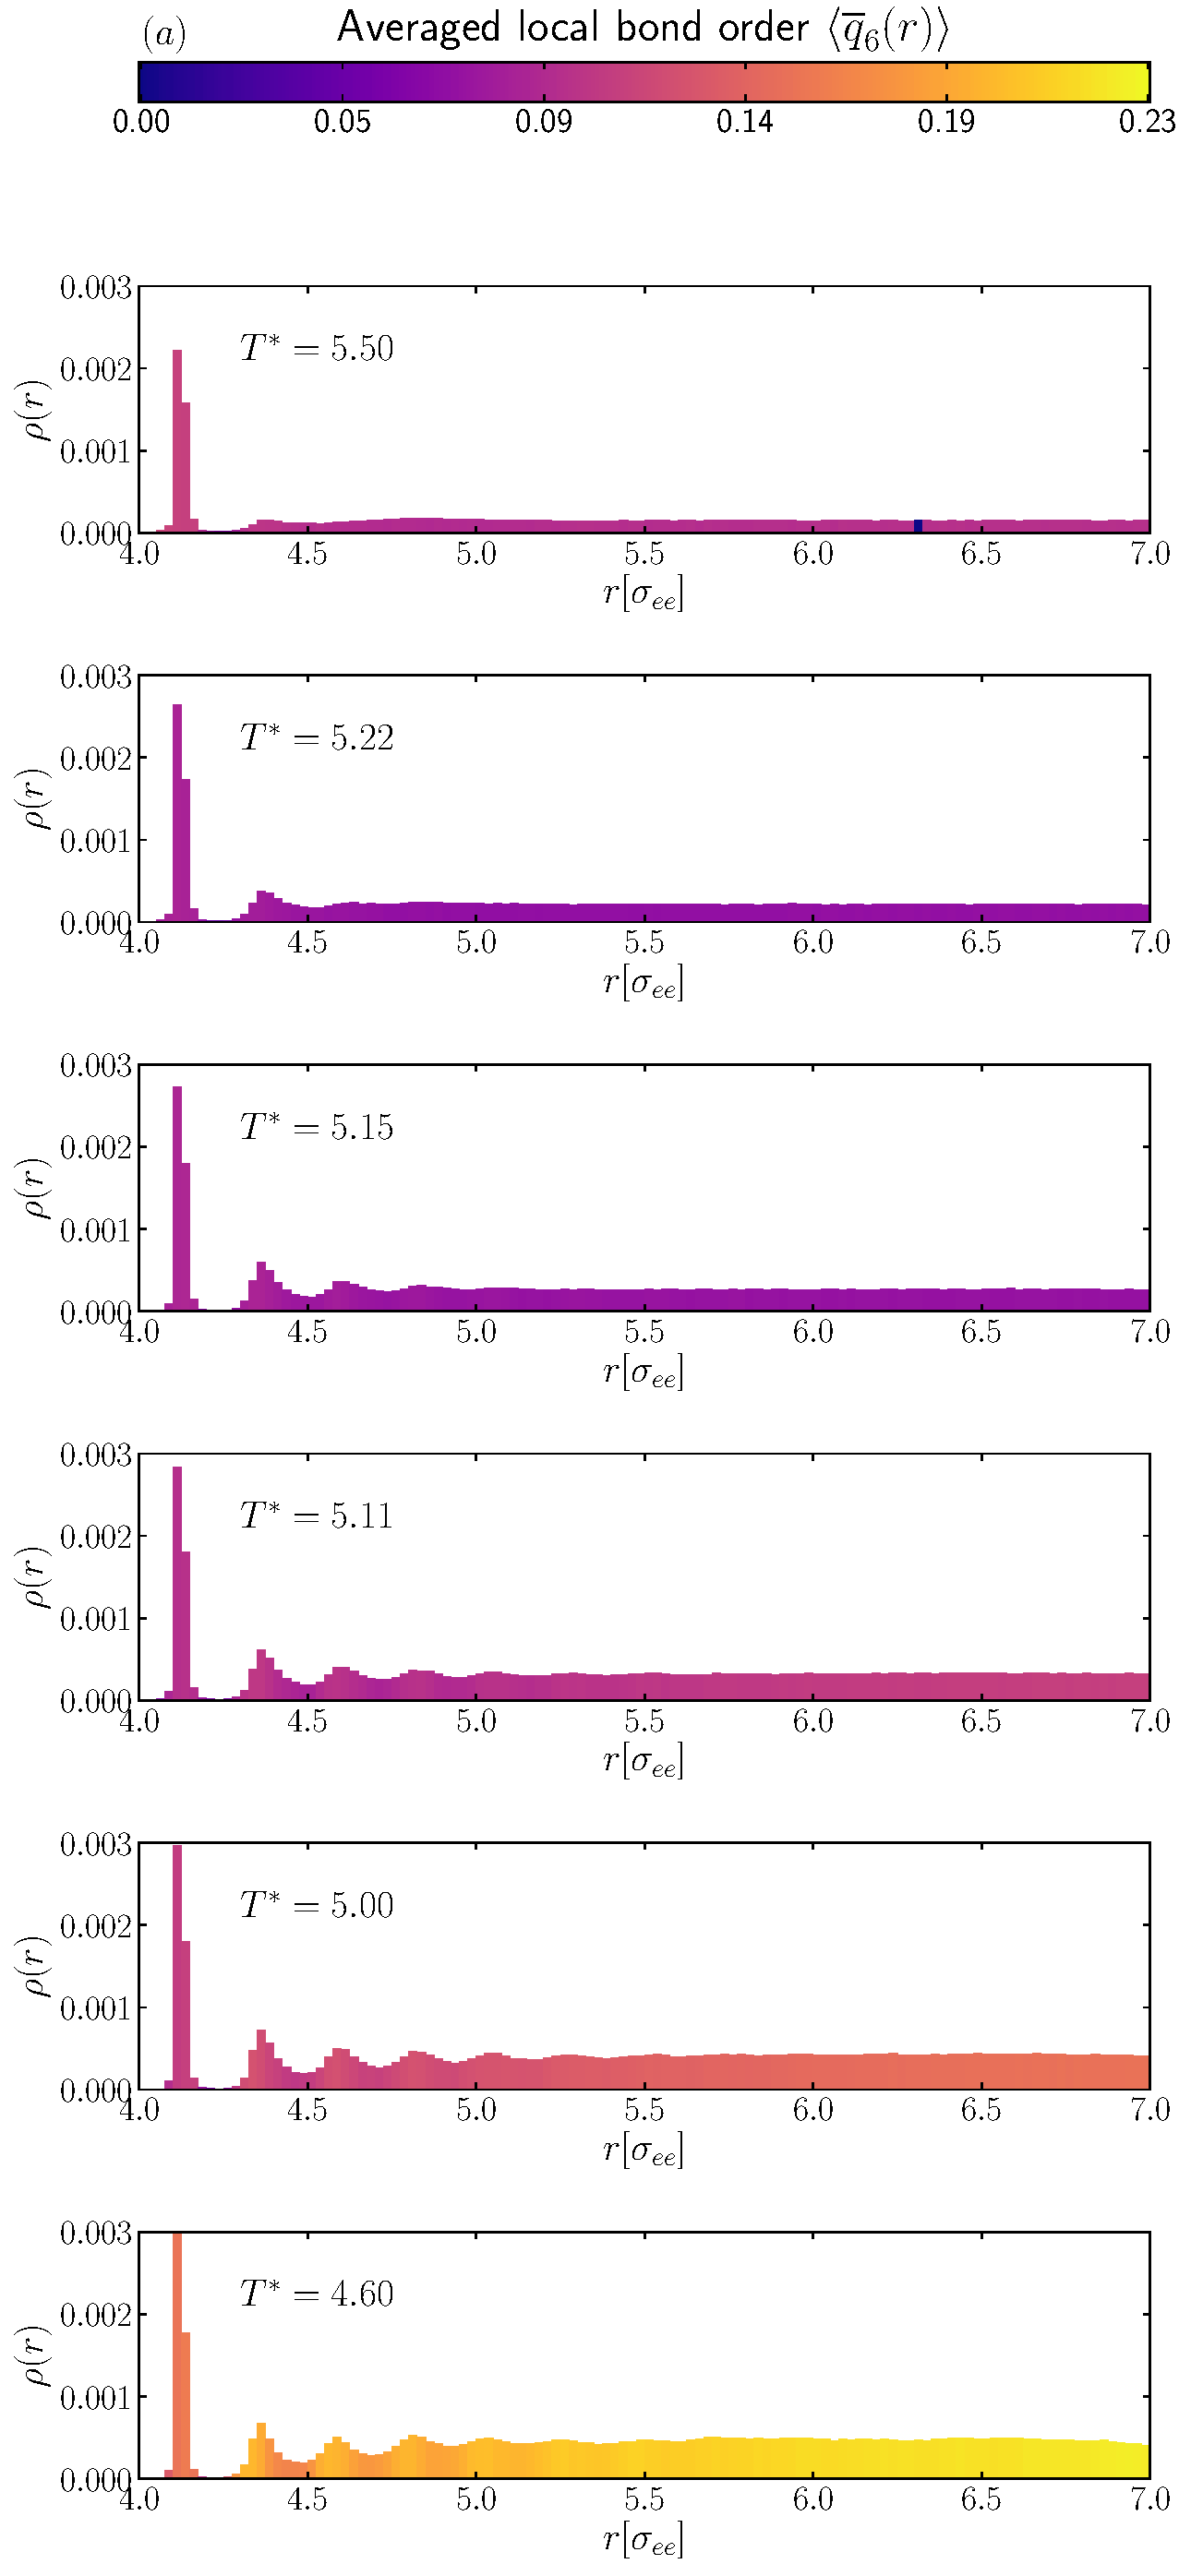
\includegraphics[width=0.49\linewidth]{plots/bfo_C56_raddensD8.pdf}
	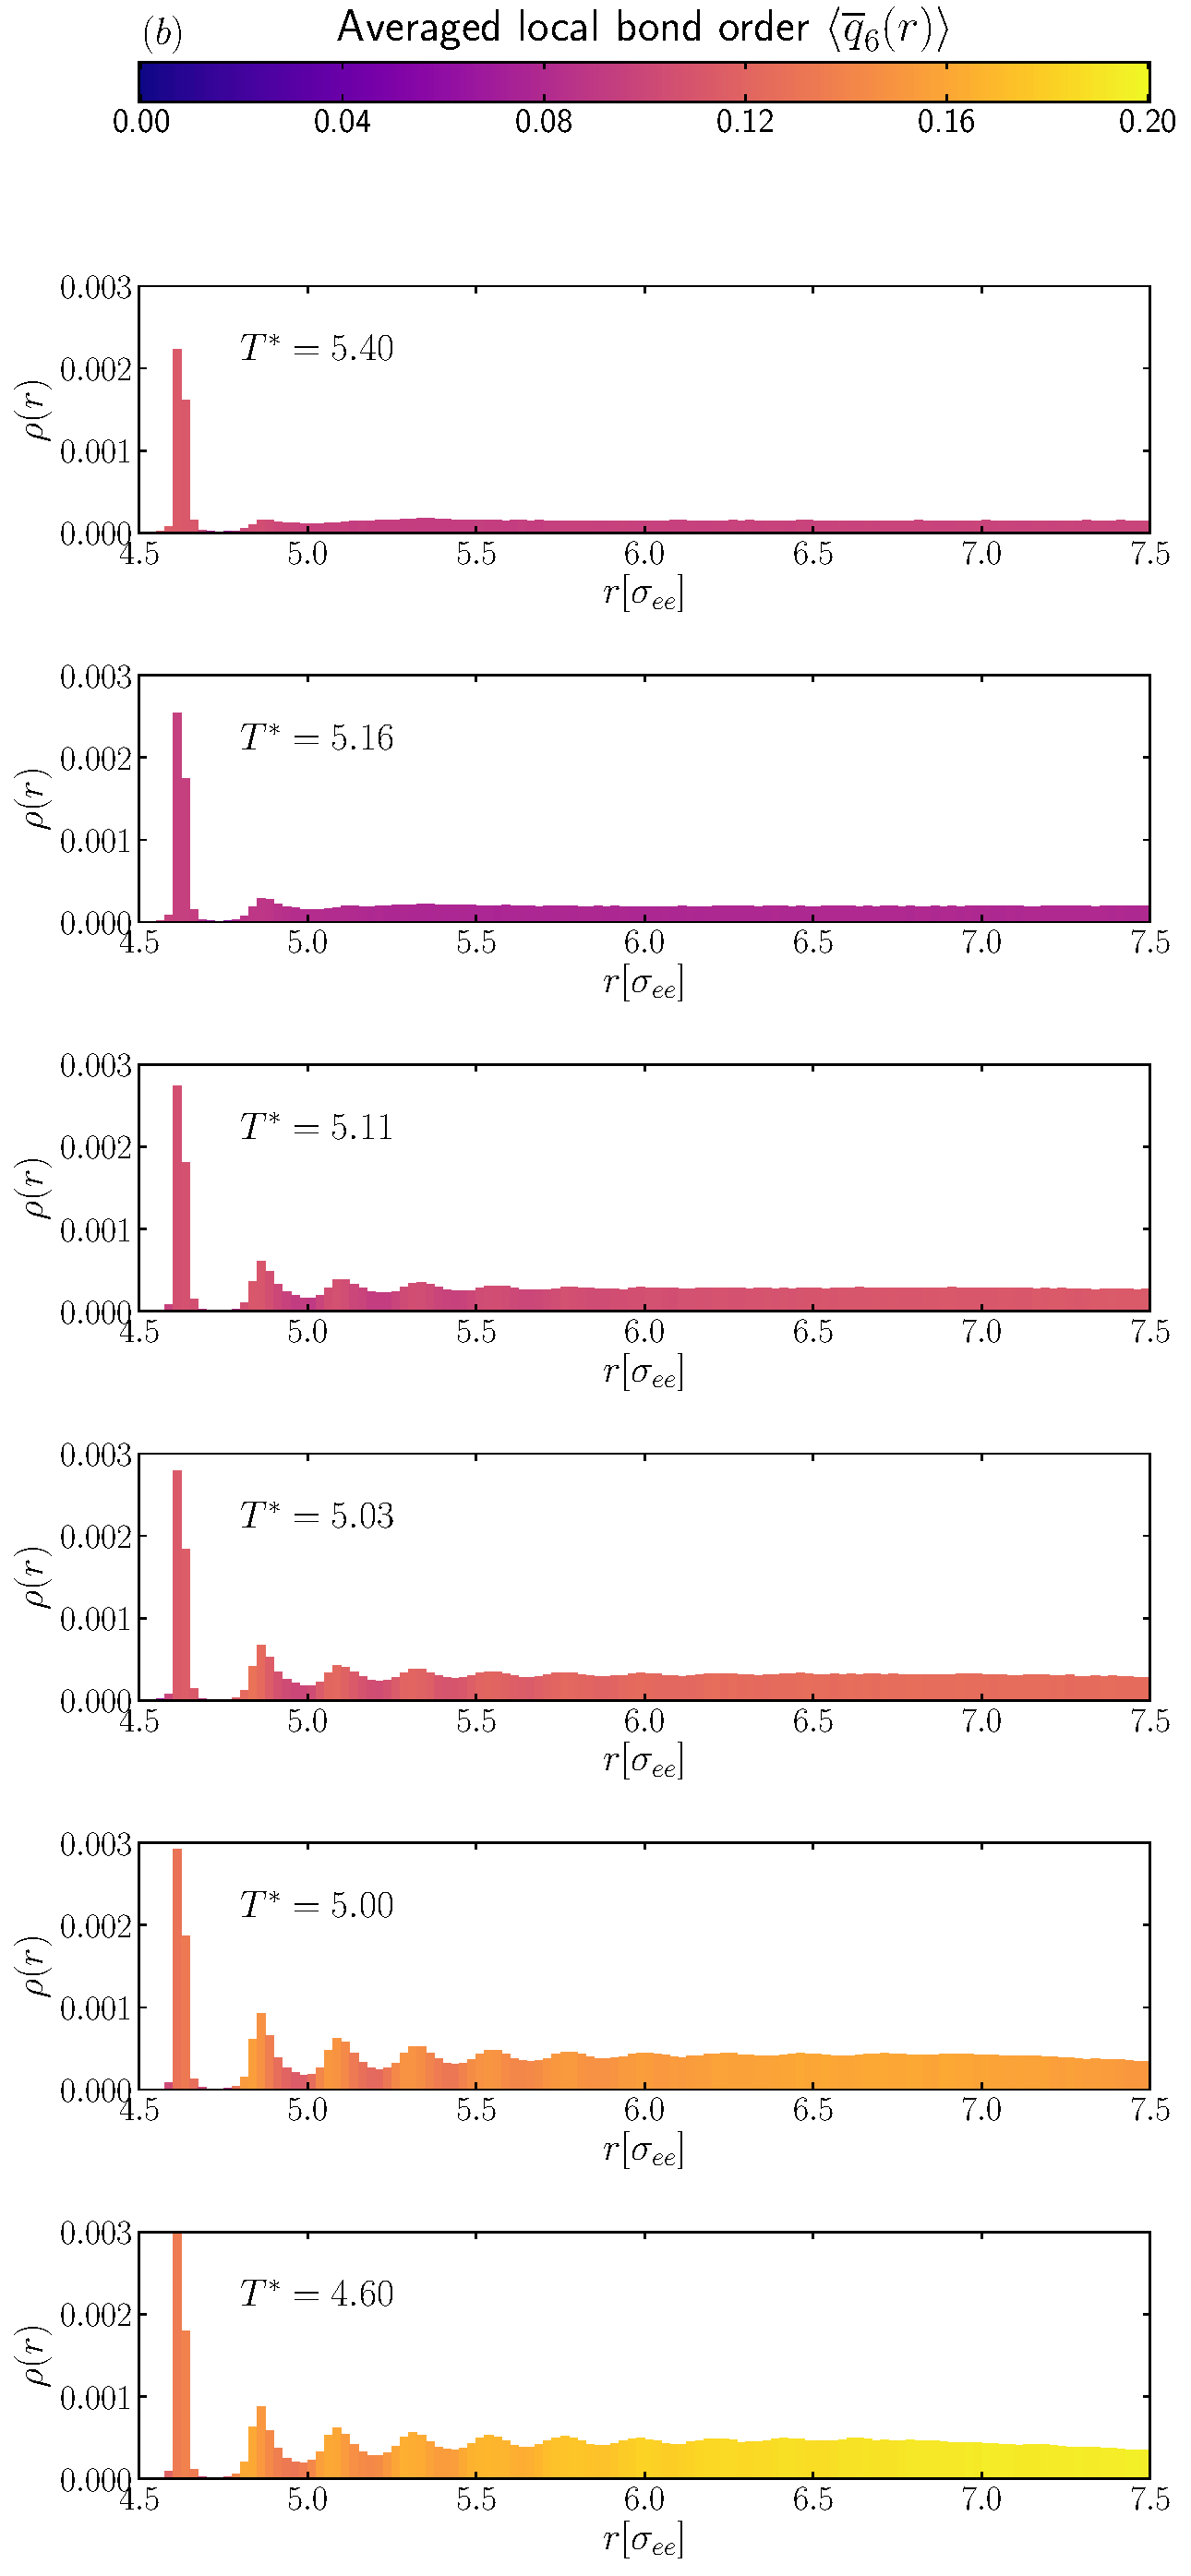
\includegraphics[width=0.49\linewidth]{plots/bfo_C56_raddensD9.pdf}
	\caption{Radial dependence of the local density and bond orientational order parameter $ \overline{q}_6$ at different temperatures of a system with colloids of sizes $D^* =  8$ (a) and $D^* = 9$ (b)}
    \label{fig:beoc32raddens}
\end{figure}

The particles form a layer around the colloid at every temperature, seen in the distinct peak at radial distance from the colloid. The particles then start forming, loose layers around the colloid in the intermediate temperatures without a distinct bond order but increasing the local nematic order. Cooling the system even further, the layers solidify, creating domains of radially aligned particles in the columnar phase.
 


